
\section{Scalability Campaign}\label{results:scale}

Given the base parameter values described in Tables \ref{tbl:front_ref_params}
and \ref{tbl:back_ref_params}, exchanges were generated by scaling the number of
reactors in the system. The smallest system modeled included five reactors. The
largest exchanges included five-hundred reactors, a value chosen because there
are approximately five-hundred reactors currently operating (437) or under
construction (71) in the world \cite{nrxtrs}. Therefore, the largest exchanges
modeled represent a time step in a simulation in which the world-wide fleet of
reactors are all supplying or consuming a batch of fuel.

Front and back-end exchanges are explored similarly in the scalability
campaign. For all 18 combinations of fundamental parameters and each solver, a
set of reference cases are established, where the only varying parameter is the
number of reactors. Both the solution time and objective value metrics are
compared as the problem size increases. Additionally, the effect of convergence
criteria for the \cbc solver is investigated.

Individual figures for each experiment are provided for each fuel cycle modeled
($f_\text{fc}$) and each solver. Each figure summarizes the results for all
combinations of $f_\text{rx}$ and $f_\text{loc}$. The layout for each six-pane
figure is shown below.

\begin{figure}[h!]
  \begin{center}
    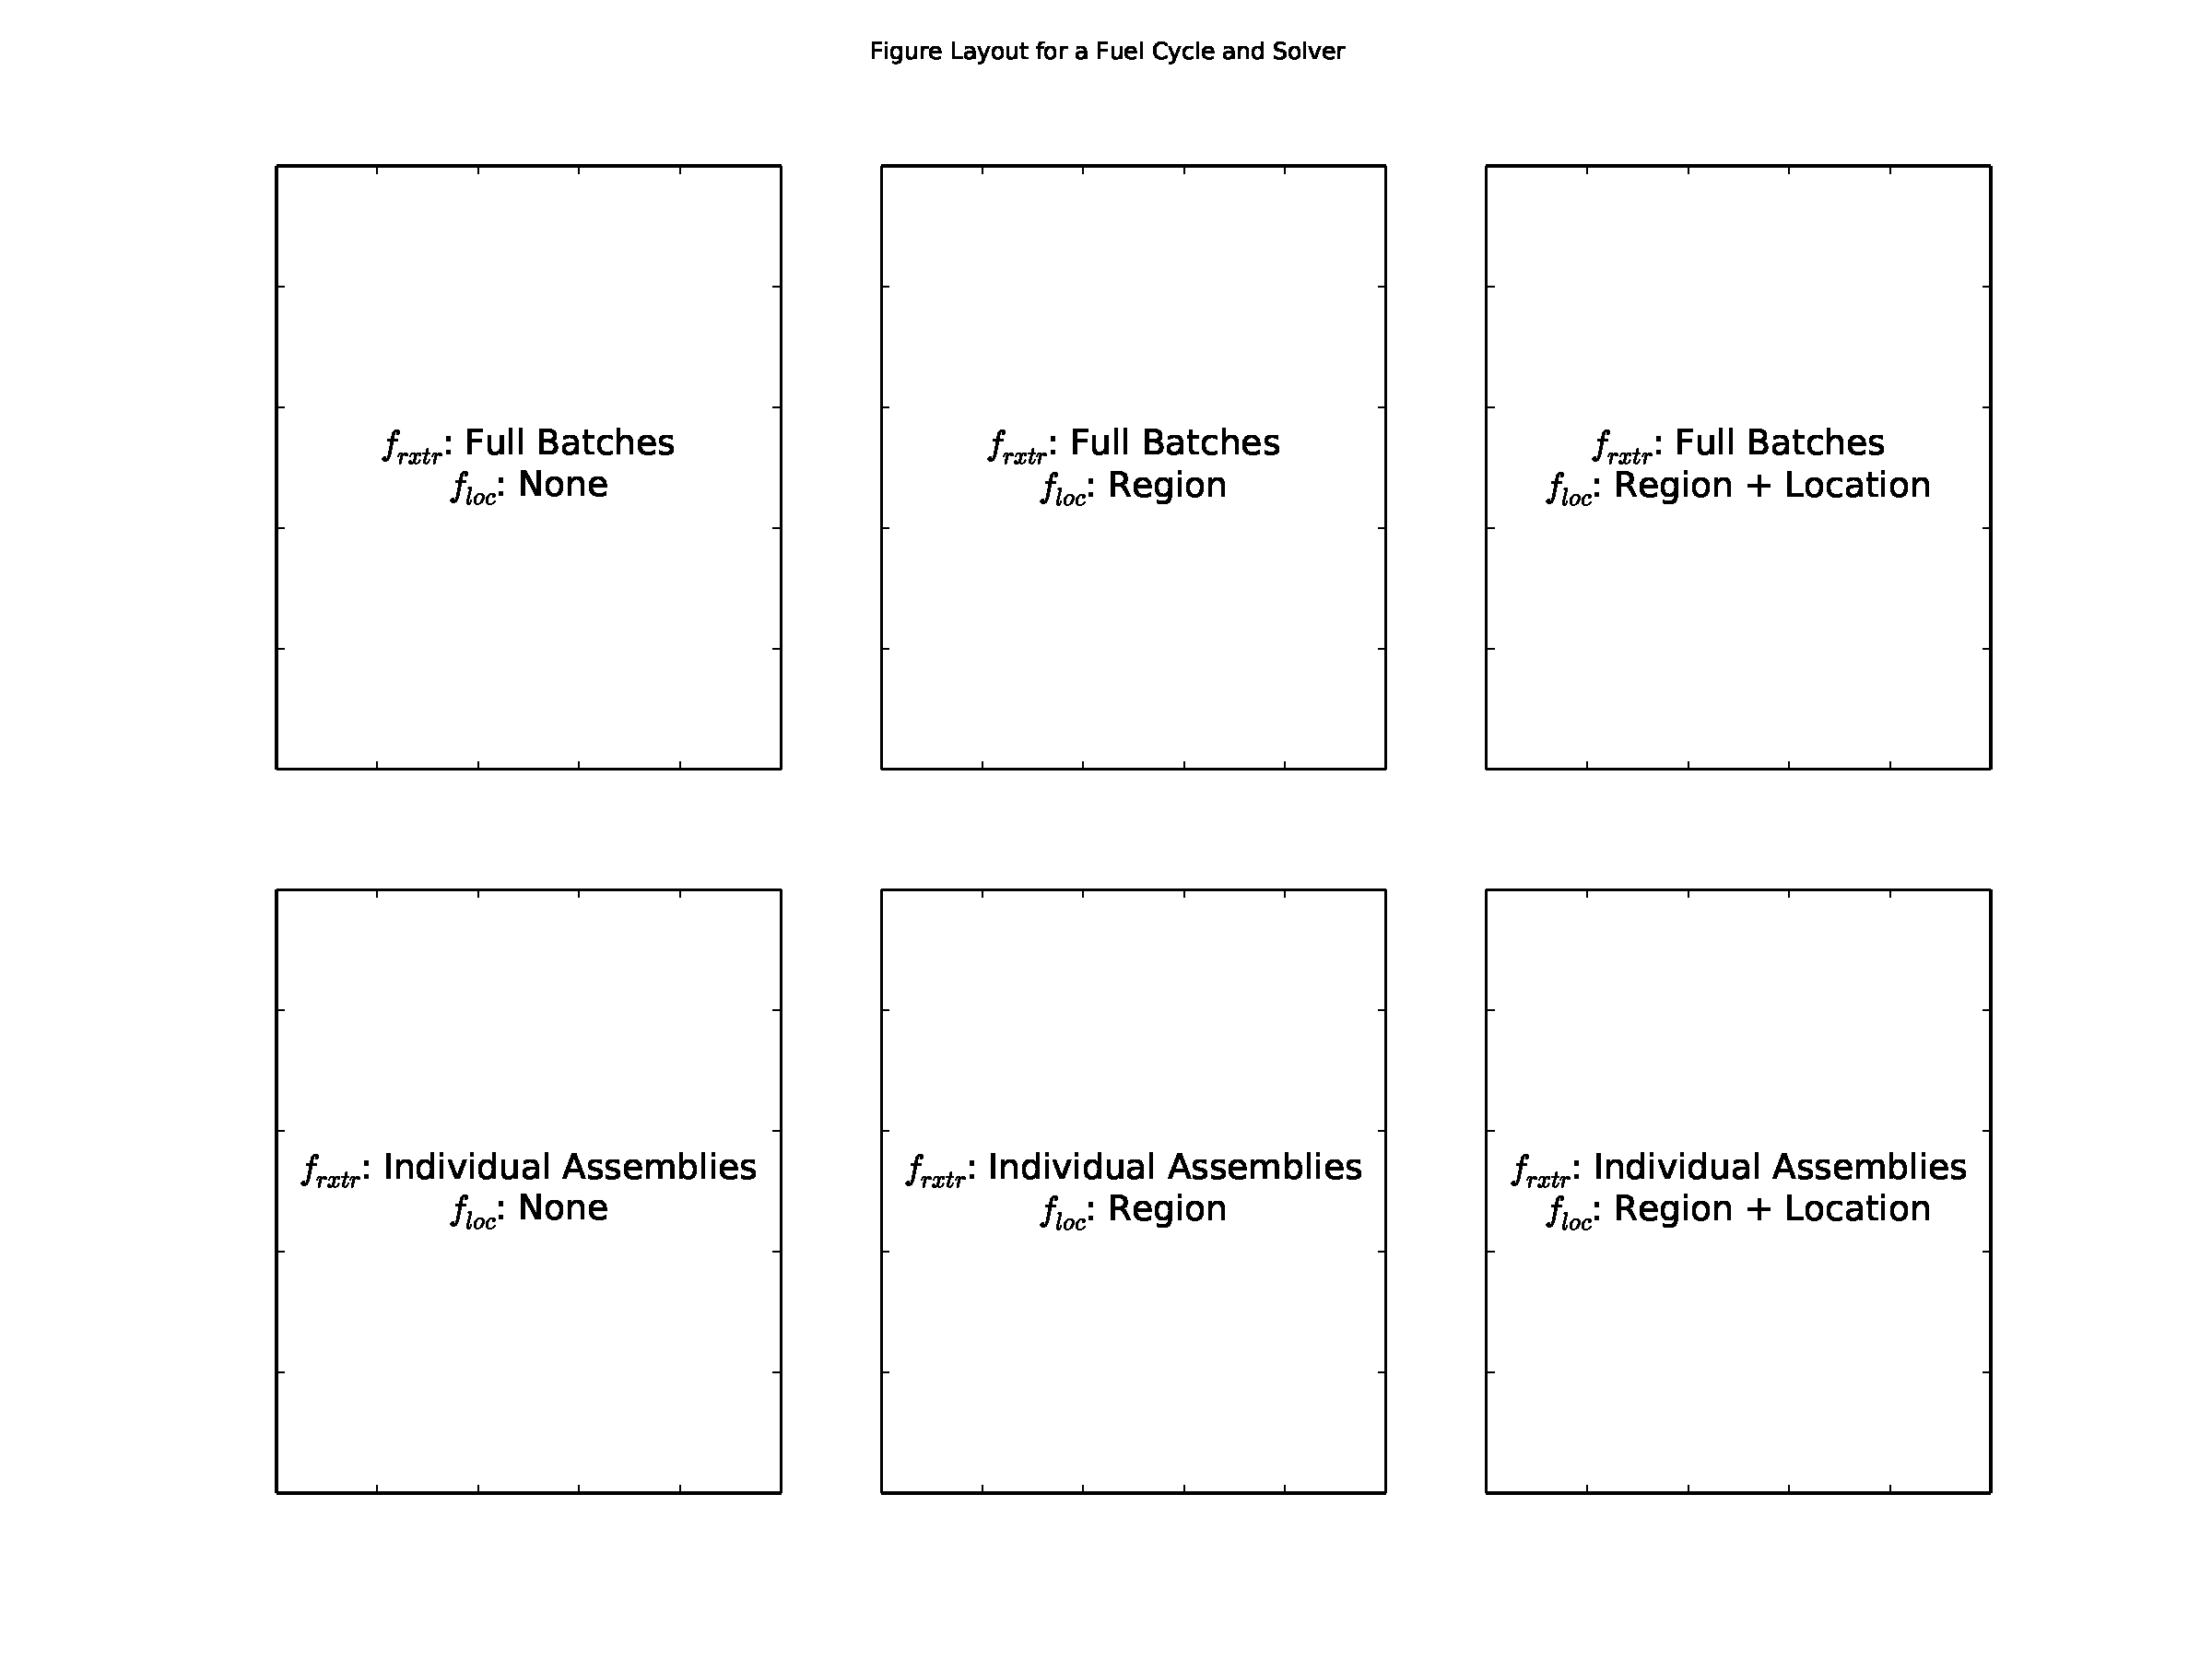
\includegraphics[width=.7\textwidth]{figure_layout.pdf}
    \caption{
      \label{fig:figure_layout}
      The general figure layout displaying results for different fundamental
      parameter values.}
  \end{center}
\end{figure}

\subsection{Front-End Exchanges}

\subsubsection{Reference Case}

Reference cases were generated for front-end exchanges by scaling the number of
reactors in each exchange. A step size of 5 reactors was used for the range of
$[5, 100]$ and a step size of 25 was used from $(100, 500]$. Both the number of
  variables and number of constraints in a problem are measures of problem
  scaling. In the NFCTP, constraints are provided by trading entities, and the
  number of variables is equal to the number of arcs in a given exchange
  graph. Accordingly, understanding how each quantity scales with the number of
  reactors is important.

Figure \ref{fig:base_front_n_rxtr_n_arcs_fc1_greedy} shows how the number of
arcs scale with problem size for the MOX fuel cycle, and Figure
\ref{fig:base_front_n_rxtr_n_constrs_fc1_greedy} shows the same results for the
number of constraints. The number of constraints scales linearly, for it is a
purely function of the number of entities in an exchange. However, the number of
arcs scales by $\mathcal{O}(n^2)$. During exchange generation, the number of
suppliers is a function of the number of reactors. Further, each reactor and
each supplier have an arc connecting them if the reactor can consume the
supplier's commodity. When the addition of a reactor also causes the addition of
a support facility, based on parameter vector values, arcs are added for the new
reactor and for every reactor previously existing in the system. Therefore,
there is an an $\mathcal{O}(n^2)$ relationship between reactors and arcs. Both
relationships hold true regardless of the fuel cycle being modeled, and, as can
be seen, are also independent of other fundamental parameters. The arc
population magnitude, however, is a function of $f_\text{rxtr}$. For an
$f_\text{rxtr}$ of 1, i.e., reactors order individual assemblies, the number of
arcs per reactor is $\mathcal{O}(n_a)$. When reactors order full batches, the
number of arcs per reactor is $\mathcal{O}(1)$.

\begin{figure}[h!]
  \begin{center}
    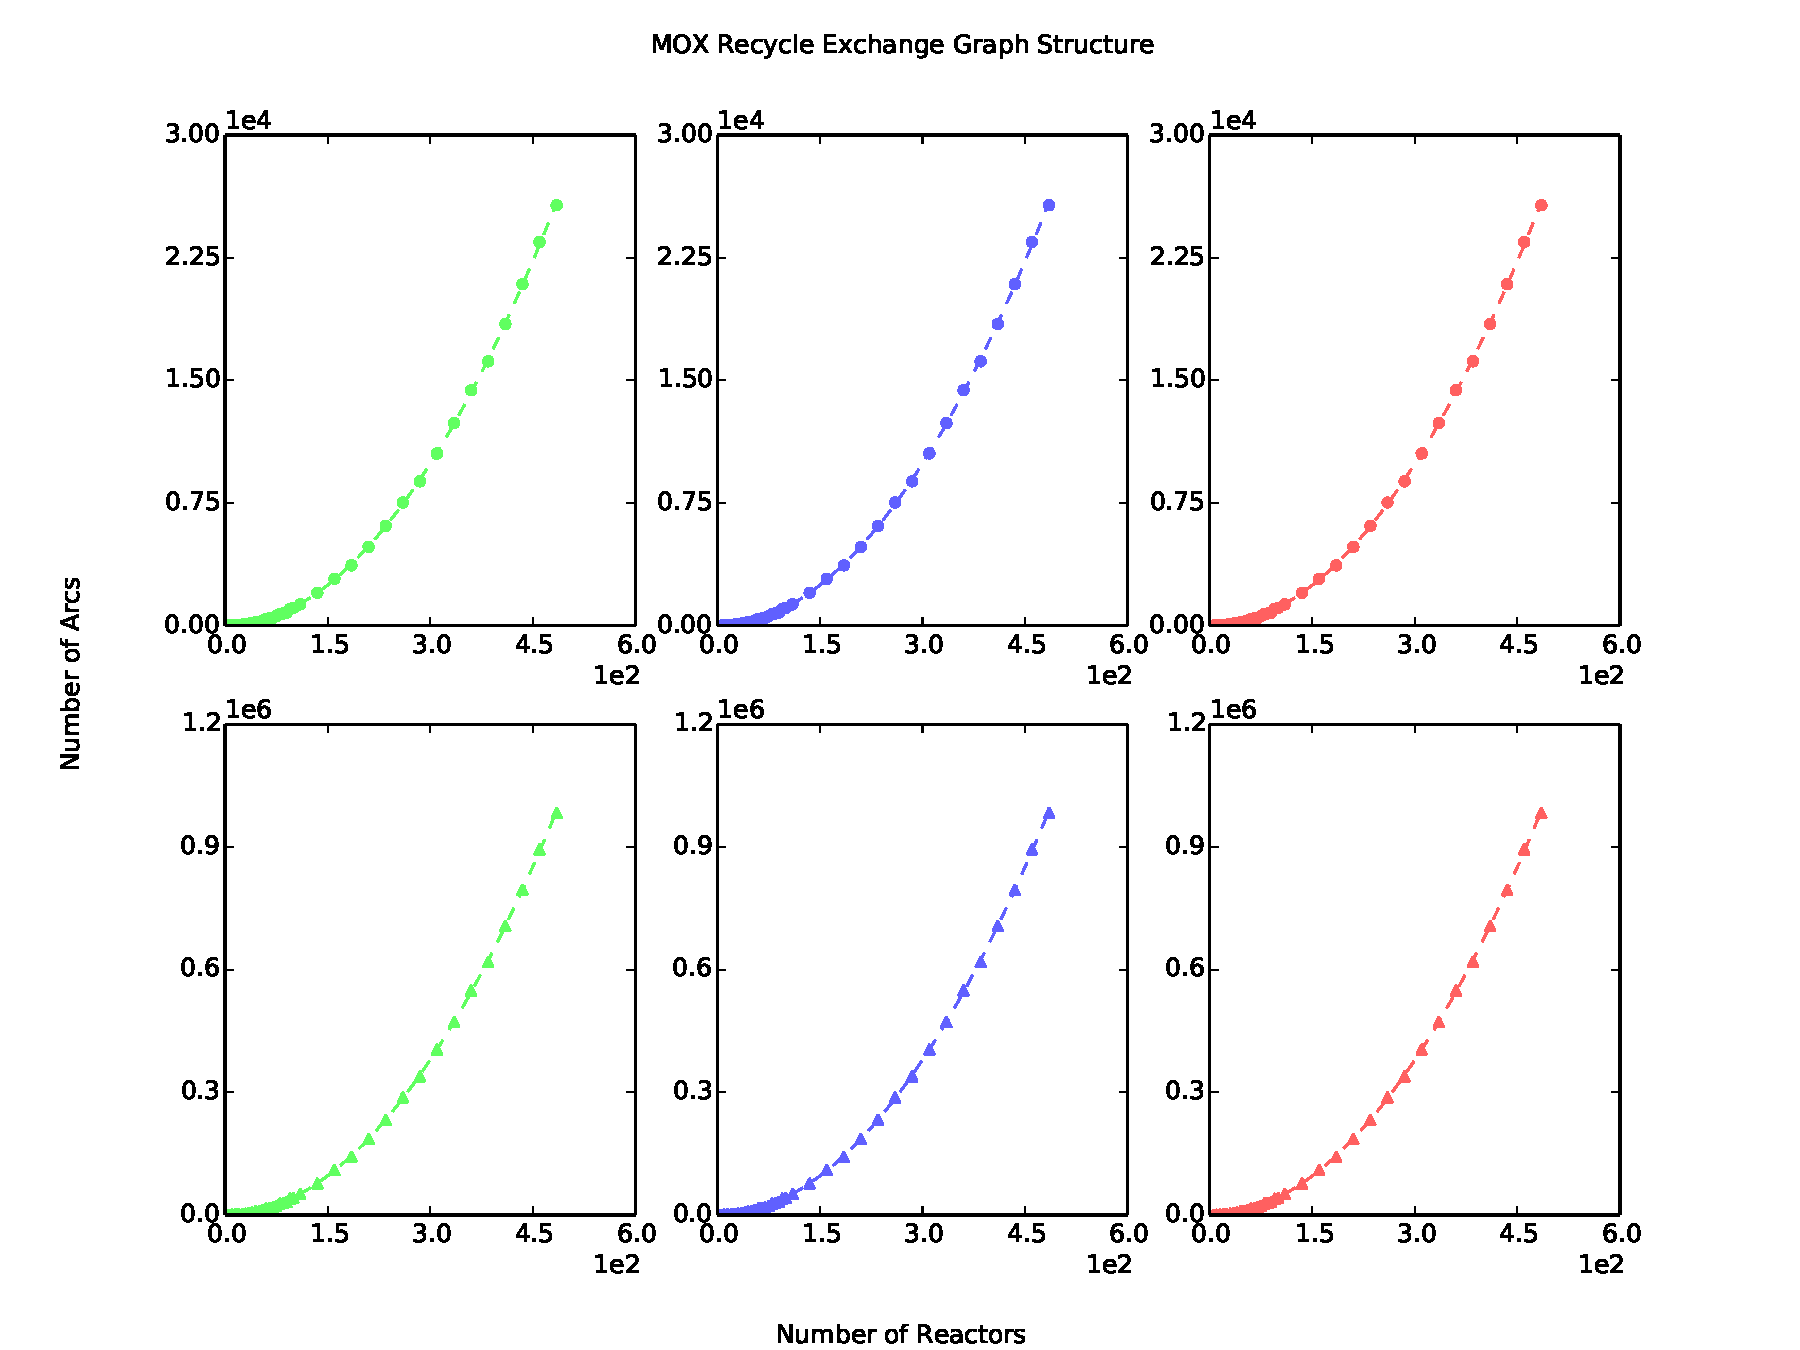
\includegraphics[width=.7\textwidth]{base_front_n_rxtr_n_arcs_fc1_greedy.pdf}
    \caption{
      \label{fig:base_front_n_rxtr_n_arcs_fc1_greedy}
      Arc population scaling with the number of reactors with corresponding
      quadratic fits.}
  \end{center}
\end{figure}

\begin{figure}[h!]
  \begin{center}
    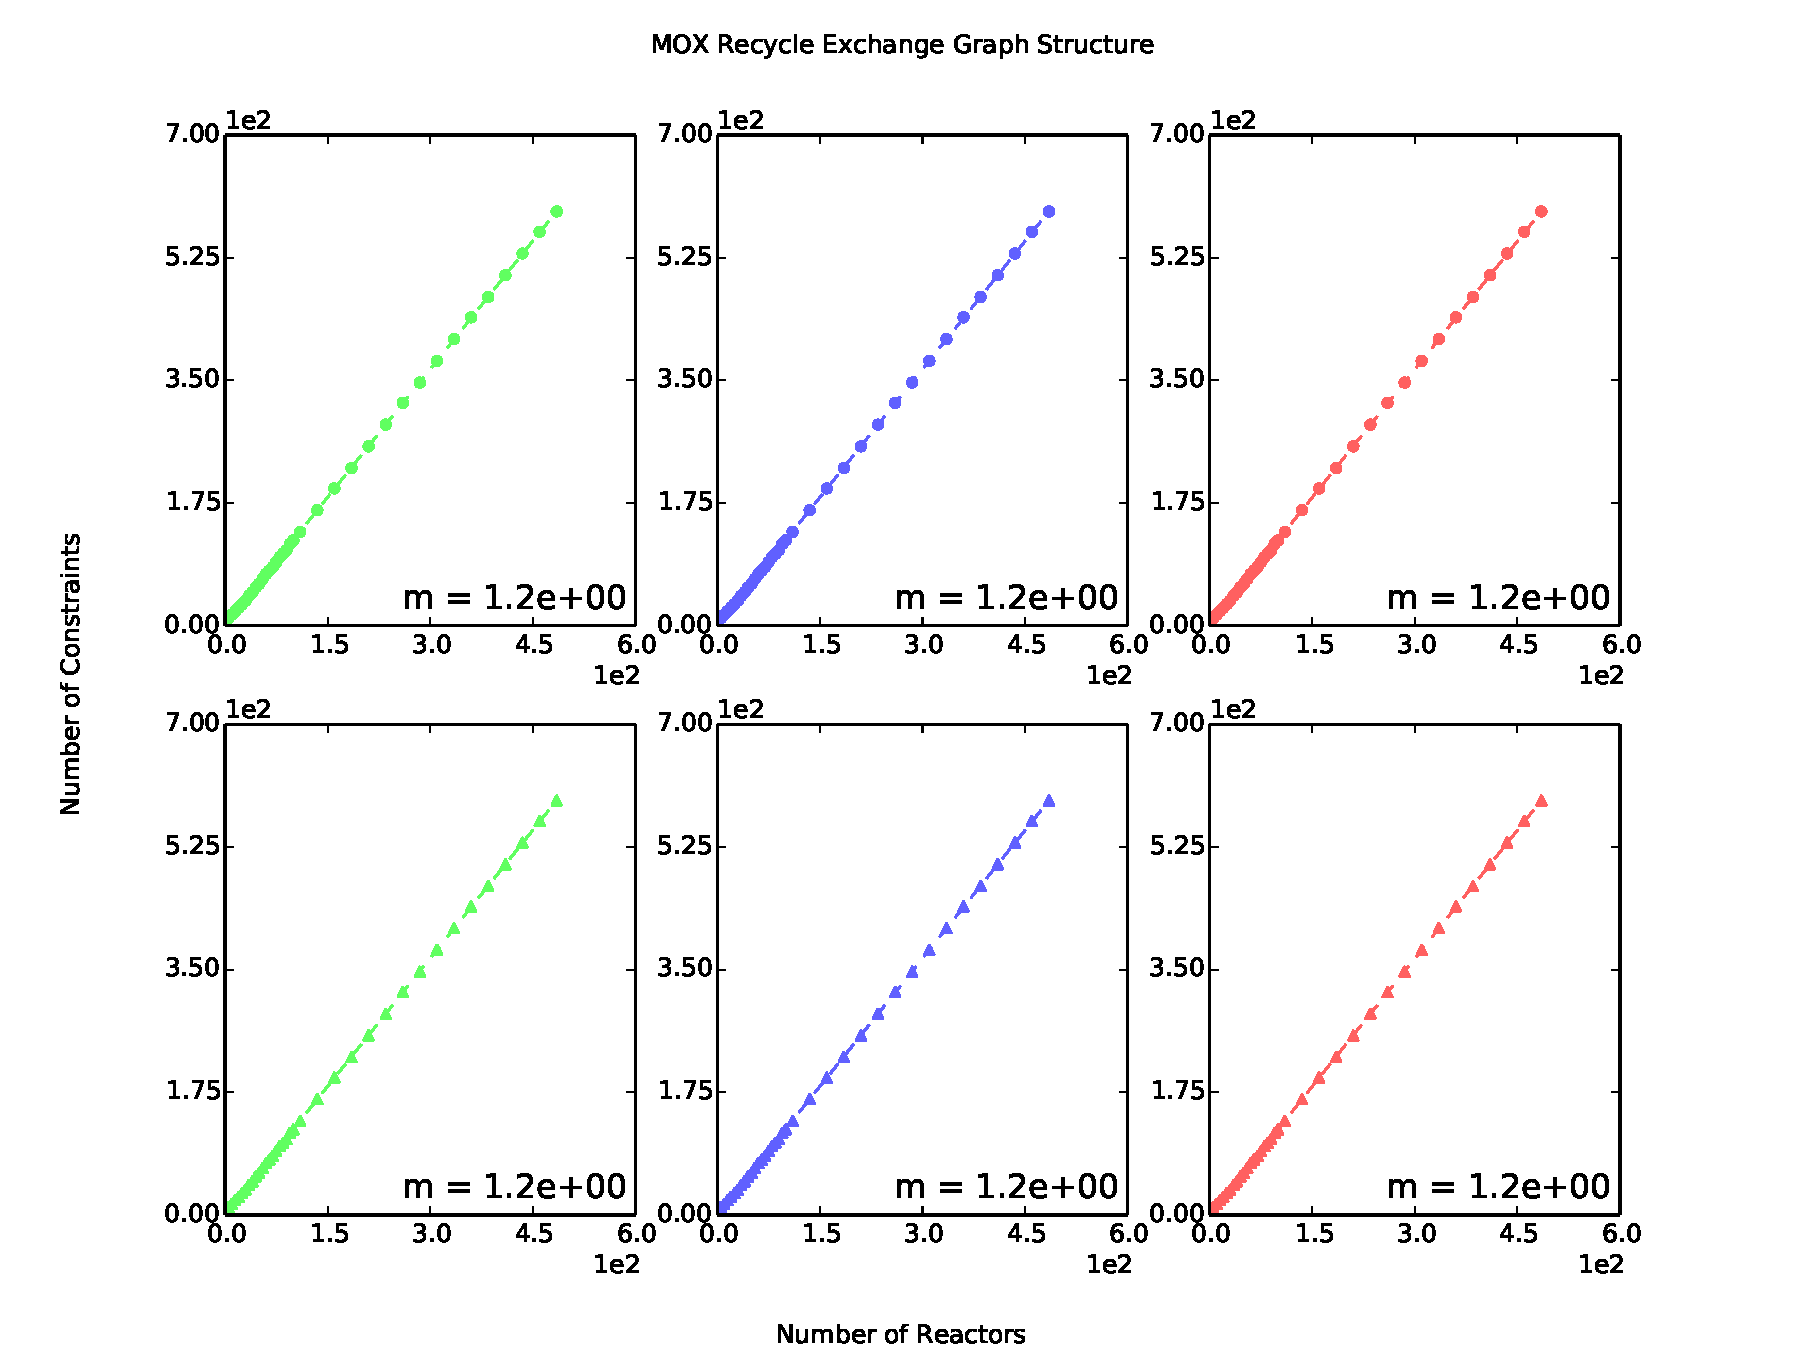
\includegraphics[width=.7\textwidth]{base_front_n_rxtr_n_constrs_fc1_greedy.pdf}
    \caption{
      \label{fig:base_front_n_rxtr_n_constrs_fc1_greedy}
      Constraint population scaling with the number of reactors with
      corresponding linear fits.}
  \end{center}
\end{figure}

\paragraph{Greedy Solver}

\cref{fig:base_front_n_arcs_time_fc0_greedy,fig:base_front_n_arcs_time_fc1_greedy,fig:base_front_n_arcs_time_fc2_greedy}
show the Greedy Solver results as the number of arcs increases for the OT, MOX,
and ThOX fuel cycles, respectively. Plotted with each data set is a linear fit
with associated slope value. As discussed in \secref{results:setup}, one expects
linear-like scaling, which is observed in practice. This scaling behavior is
consistent across all fundamental parameters. Of note, however, is that the
scaling constant does increase when moving from low-fidelity reactor models to
higher-fidelity models.

\begin{figure}[h!]
  \begin{center}
    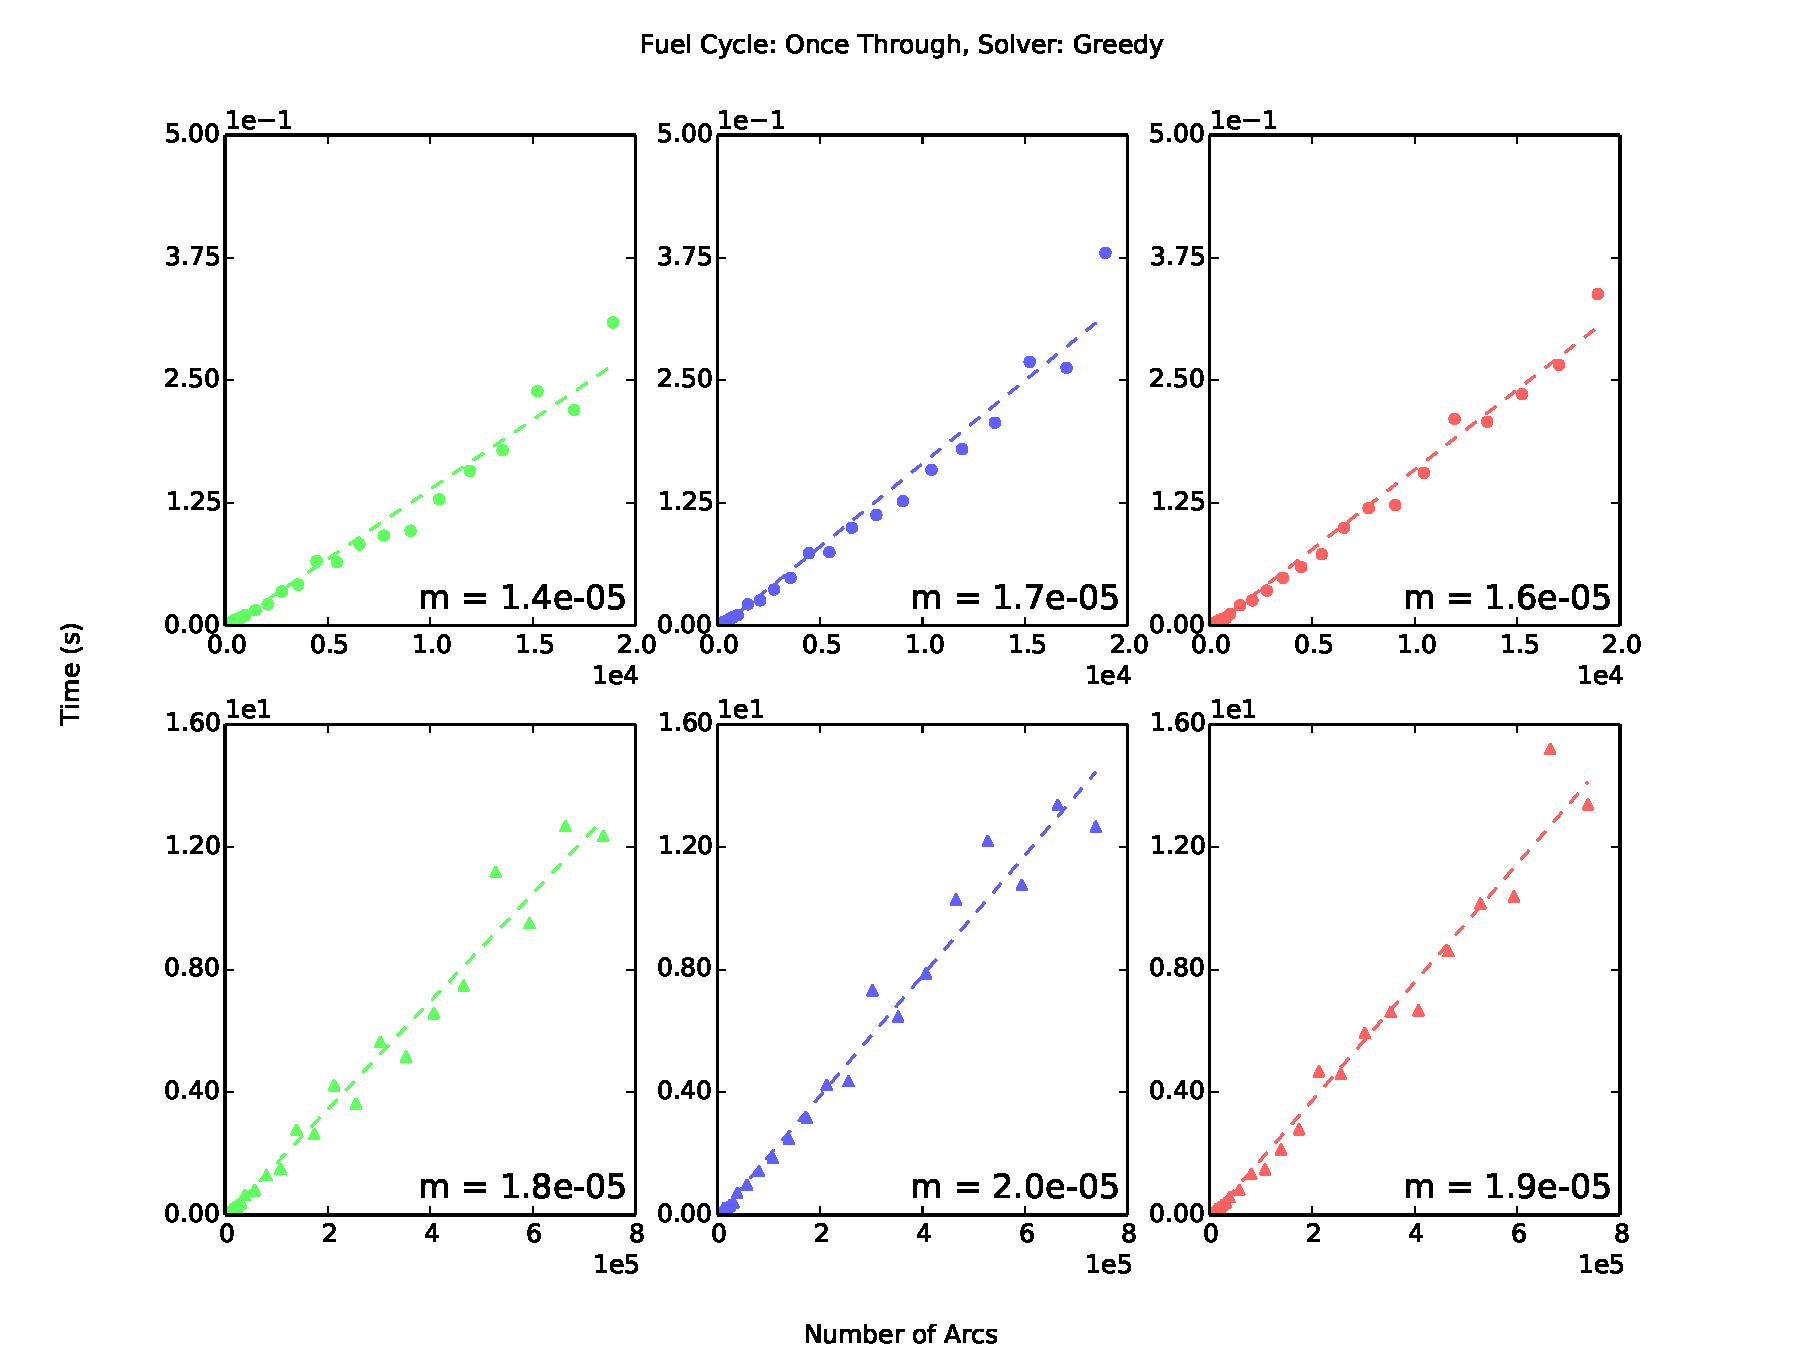
\includegraphics[width=.7\textwidth]{base_front_n_arcs_time_fc0_greedy.pdf}
    \caption{
      \label{fig:base_front_n_arcs_time_fc0_greedy}
      Greedy Solver results for the OT fuel cycle as the number of arcs
      increases.  }
  \end{center}
\end{figure}

\begin{figure}[h!]
  \begin{center}
    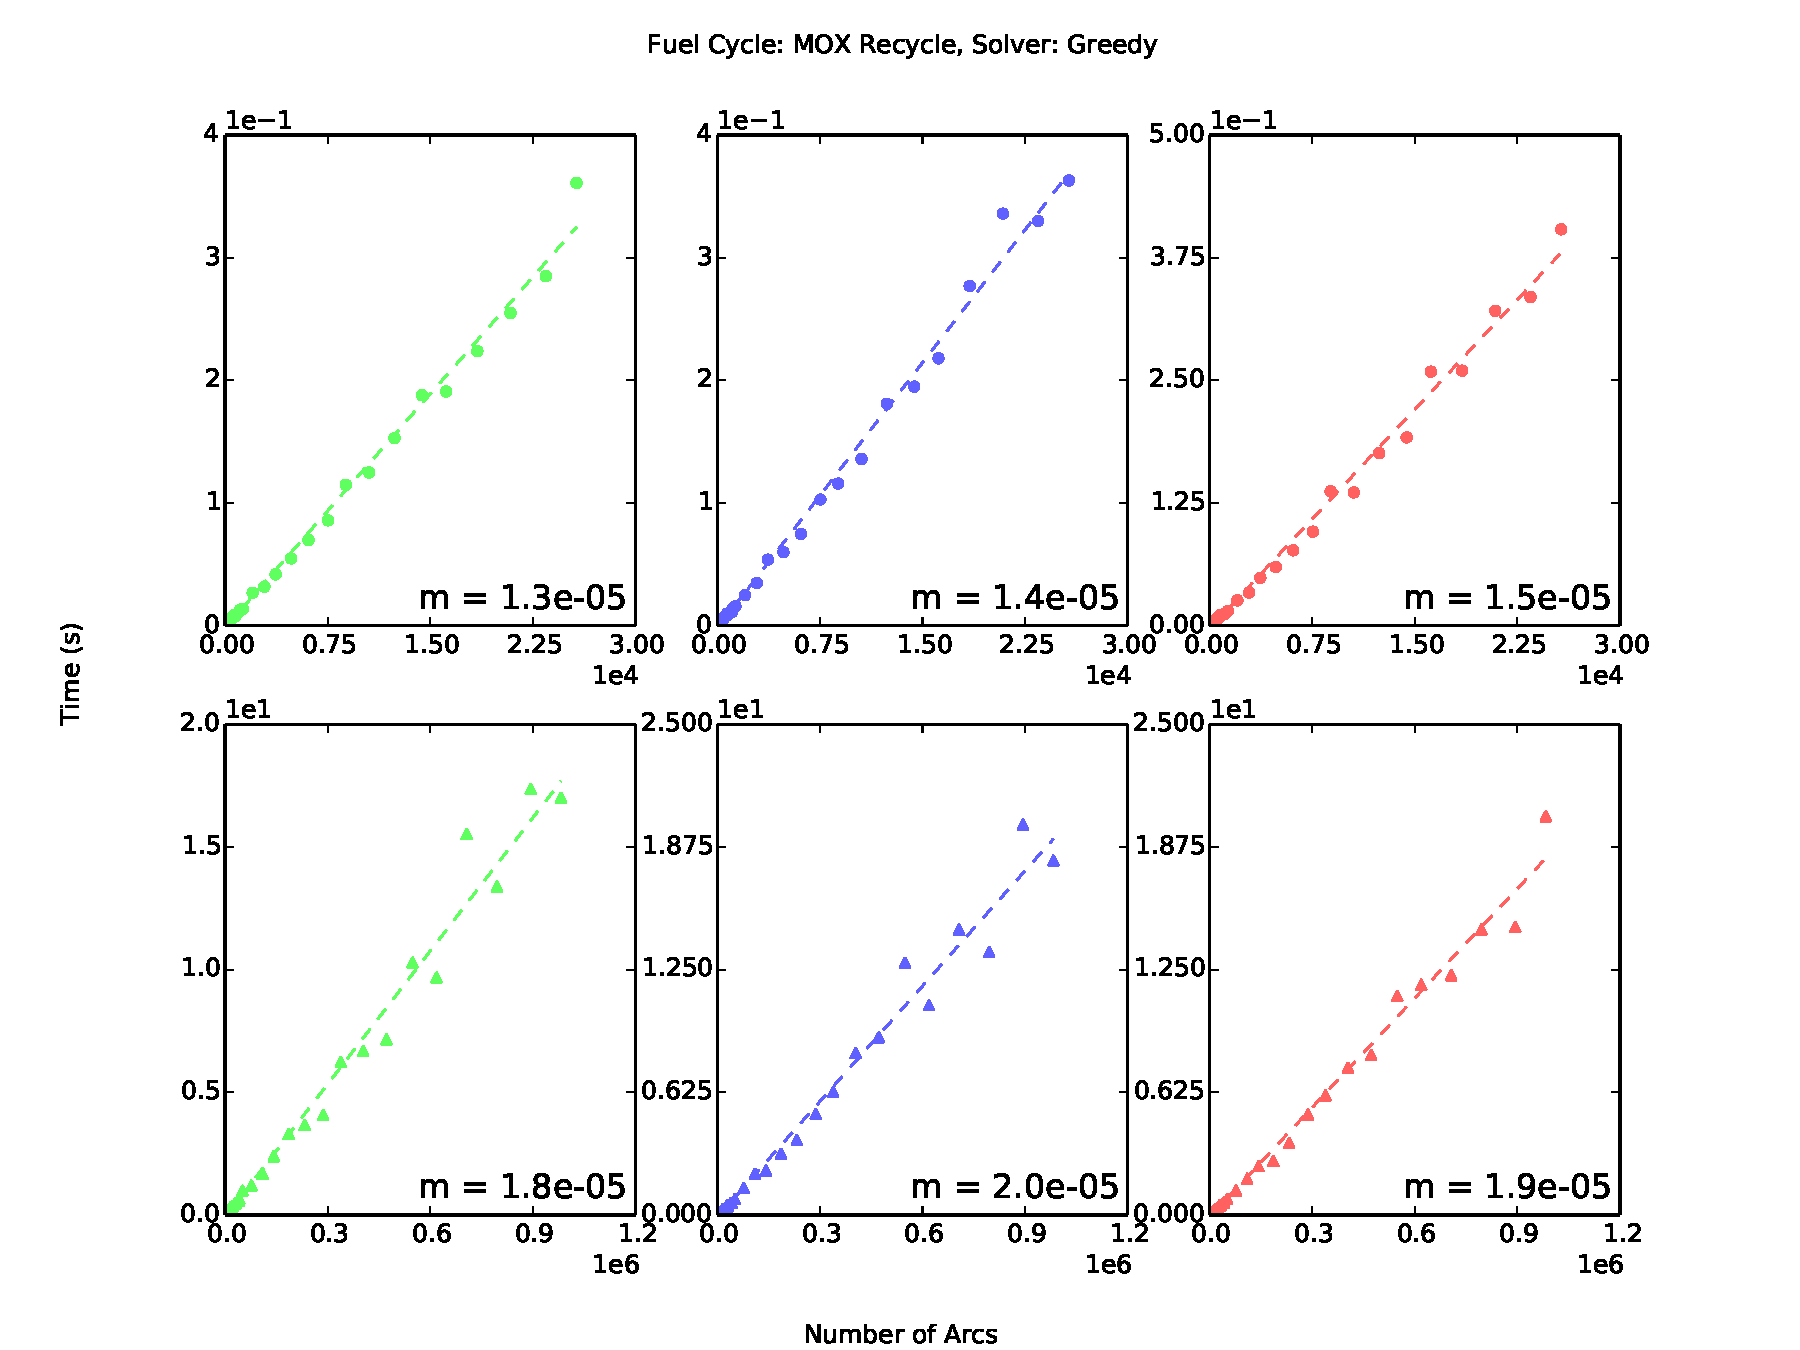
\includegraphics[width=.7\textwidth]{base_front_n_arcs_time_fc1_greedy.pdf}
    \caption{
      \label{fig:base_front_n_arcs_time_fc1_greedy}
      Greedy Solver results for the MOX fuel cycle as the number of arcs
      increases.
    }
  \end{center}
\end{figure}

\begin{figure}[h!]
  \begin{center}
    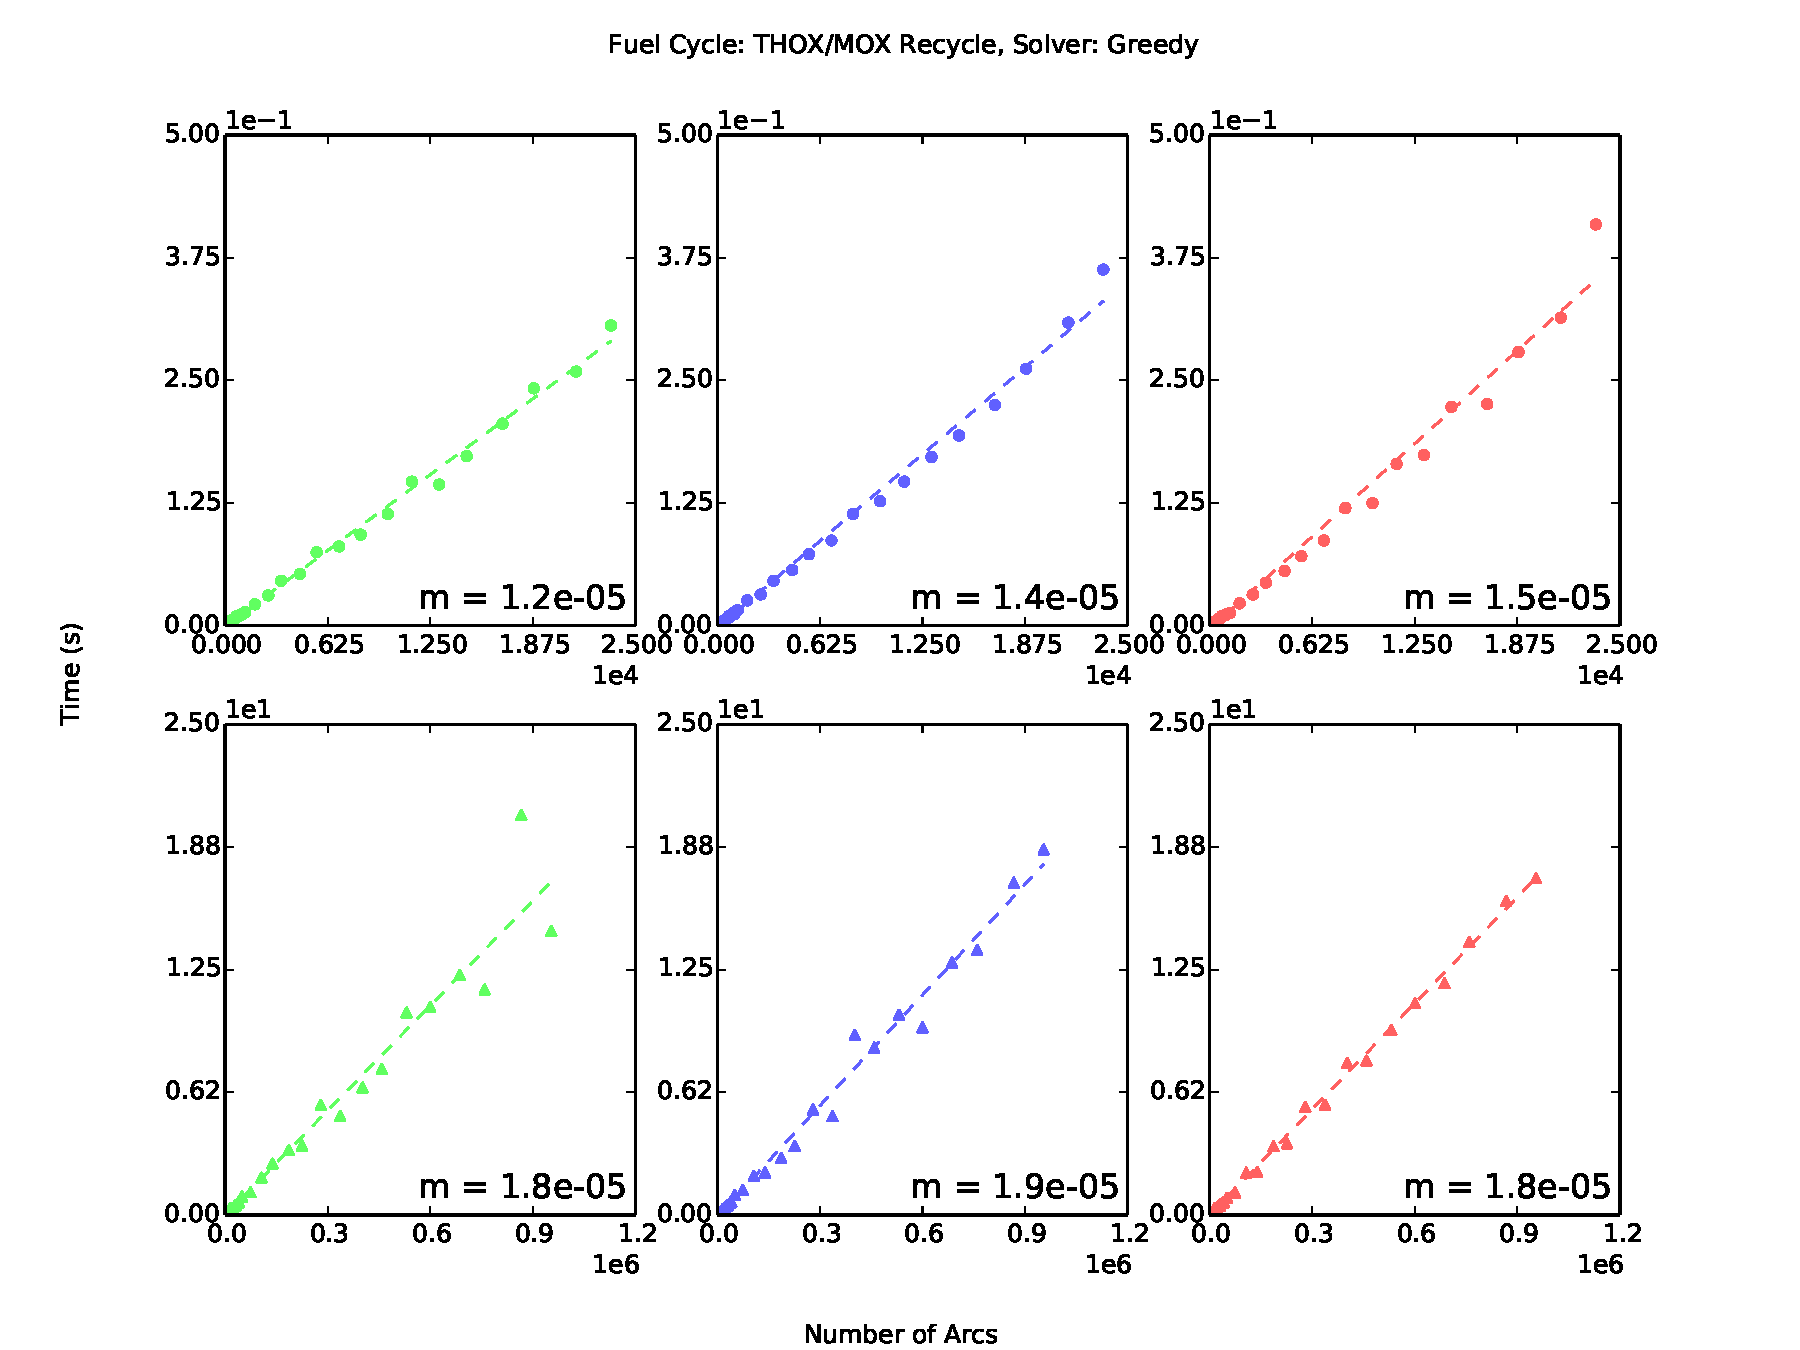
\includegraphics[width=.7\textwidth]{base_front_n_arcs_time_fc2_greedy.pdf}
    \caption{
      \label{fig:base_front_n_arcs_time_fc2_greedy}
      Greedy Solver results for the ThOX fuel cycle as the number of arcs
      increases.
      }
  \end{center}
\end{figure}

\paragraph{CLP Solver}

As discussed in \secref{results:setup}, LP solution scaling is more naturally
observed as a function of the number of
constraints. \Cref{fig:base_front_n_constrs_time_fc0_clp,fig:base_front_n_constrs_time_fc1_clp,fig:base_front_n_constrs_time_fc2_clp}
show the CLP solution times as the number of constraints increases. As can be
seen, approximate $\mathcal{O}(n^2)$ scaling is observed. Like the Greedy
solver, this scaling is independent of any fundamental paramters.

\begin{figure}[h!]
  \begin{center}
    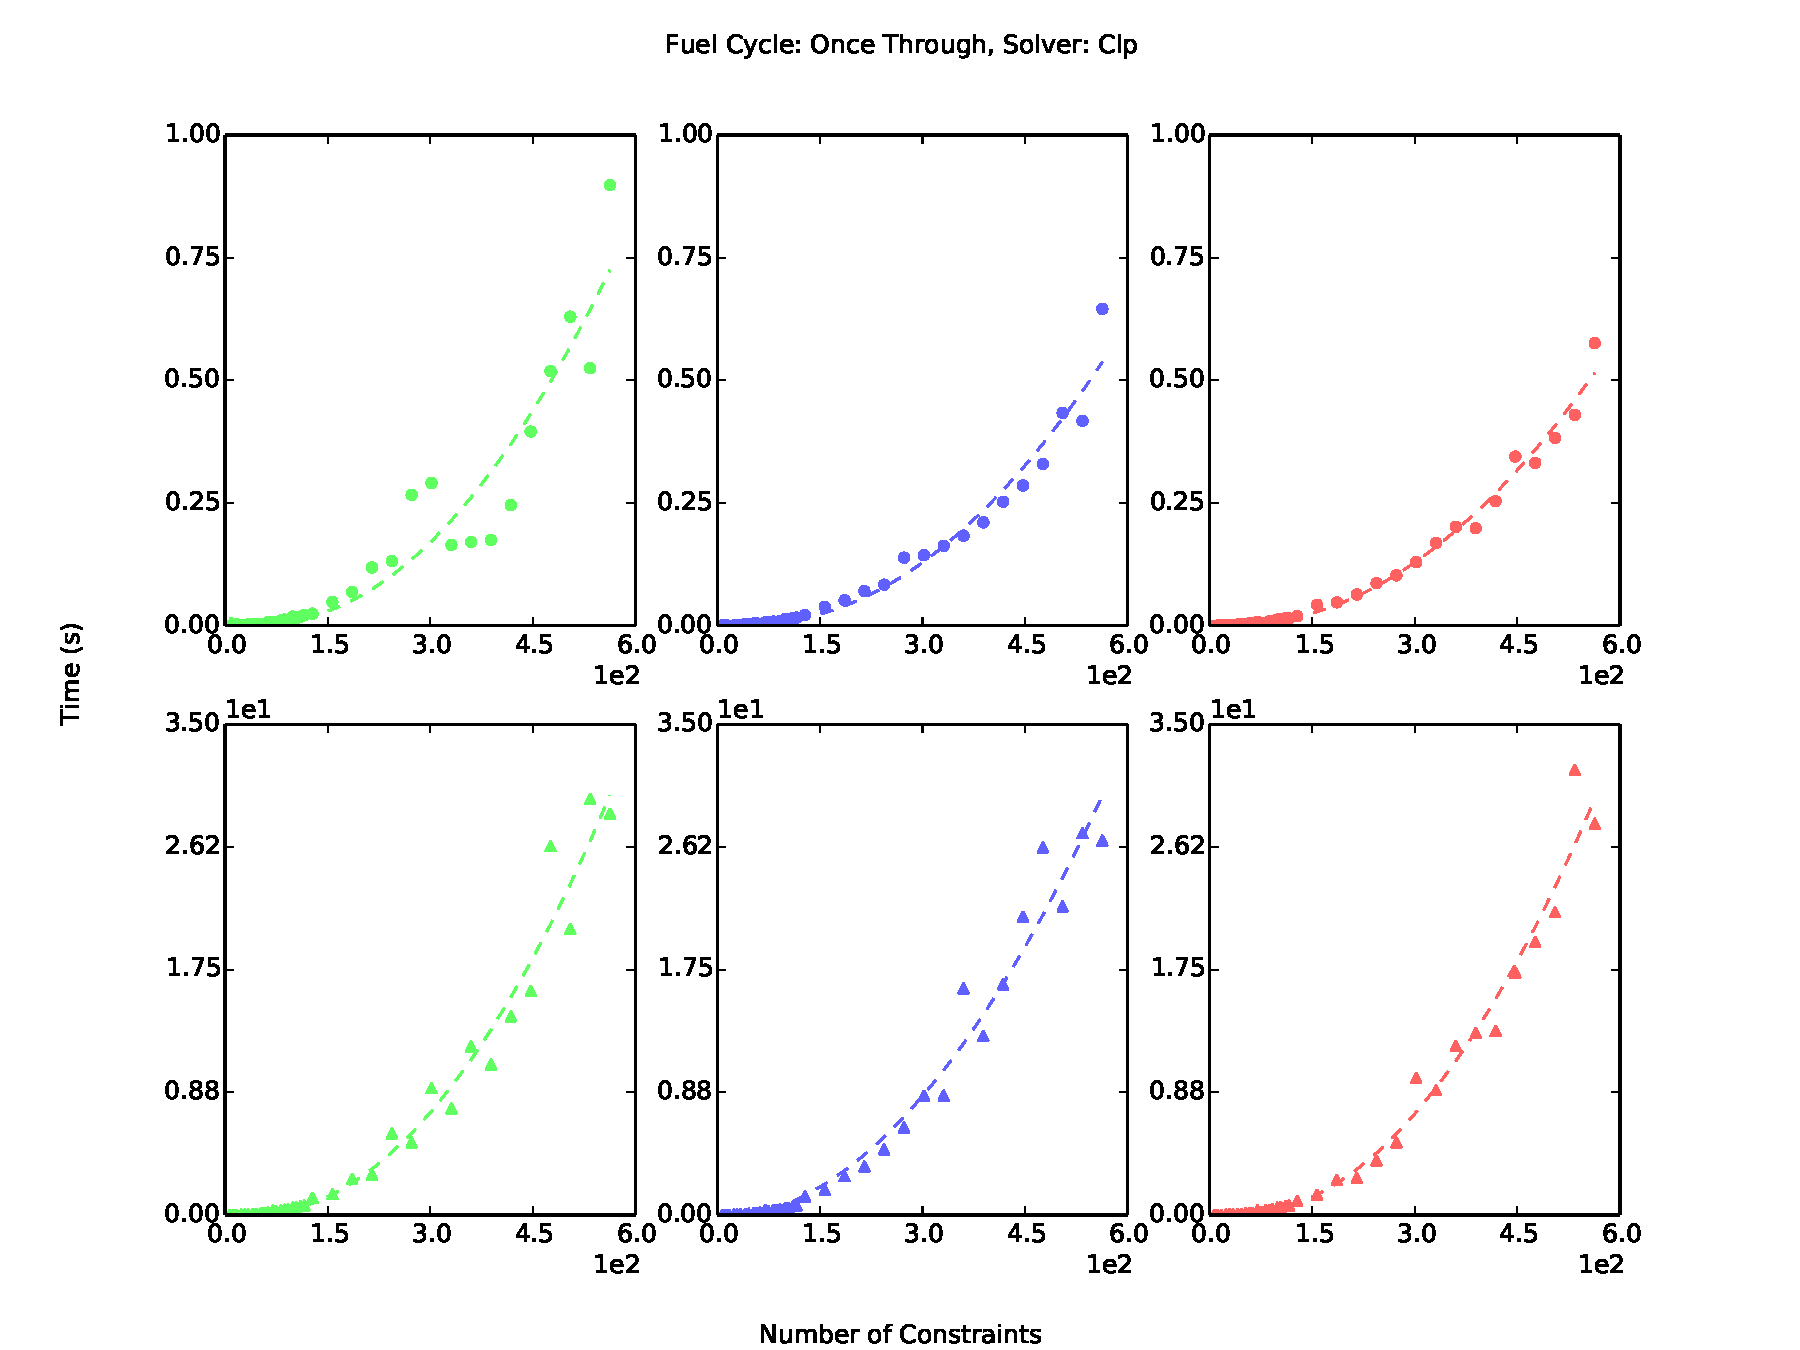
\includegraphics[width=.7\textwidth]{base_front_n_constrs_time_fc0_clp.pdf}
    \caption{
      \label{fig:base_front_n_constrs_time_fc0_clp}
      CLP Solver results for the OT fuel cycle as the number of constraints
      increases.
      }
  \end{center}
\end{figure}

\begin{figure}[h!]
  \begin{center}
    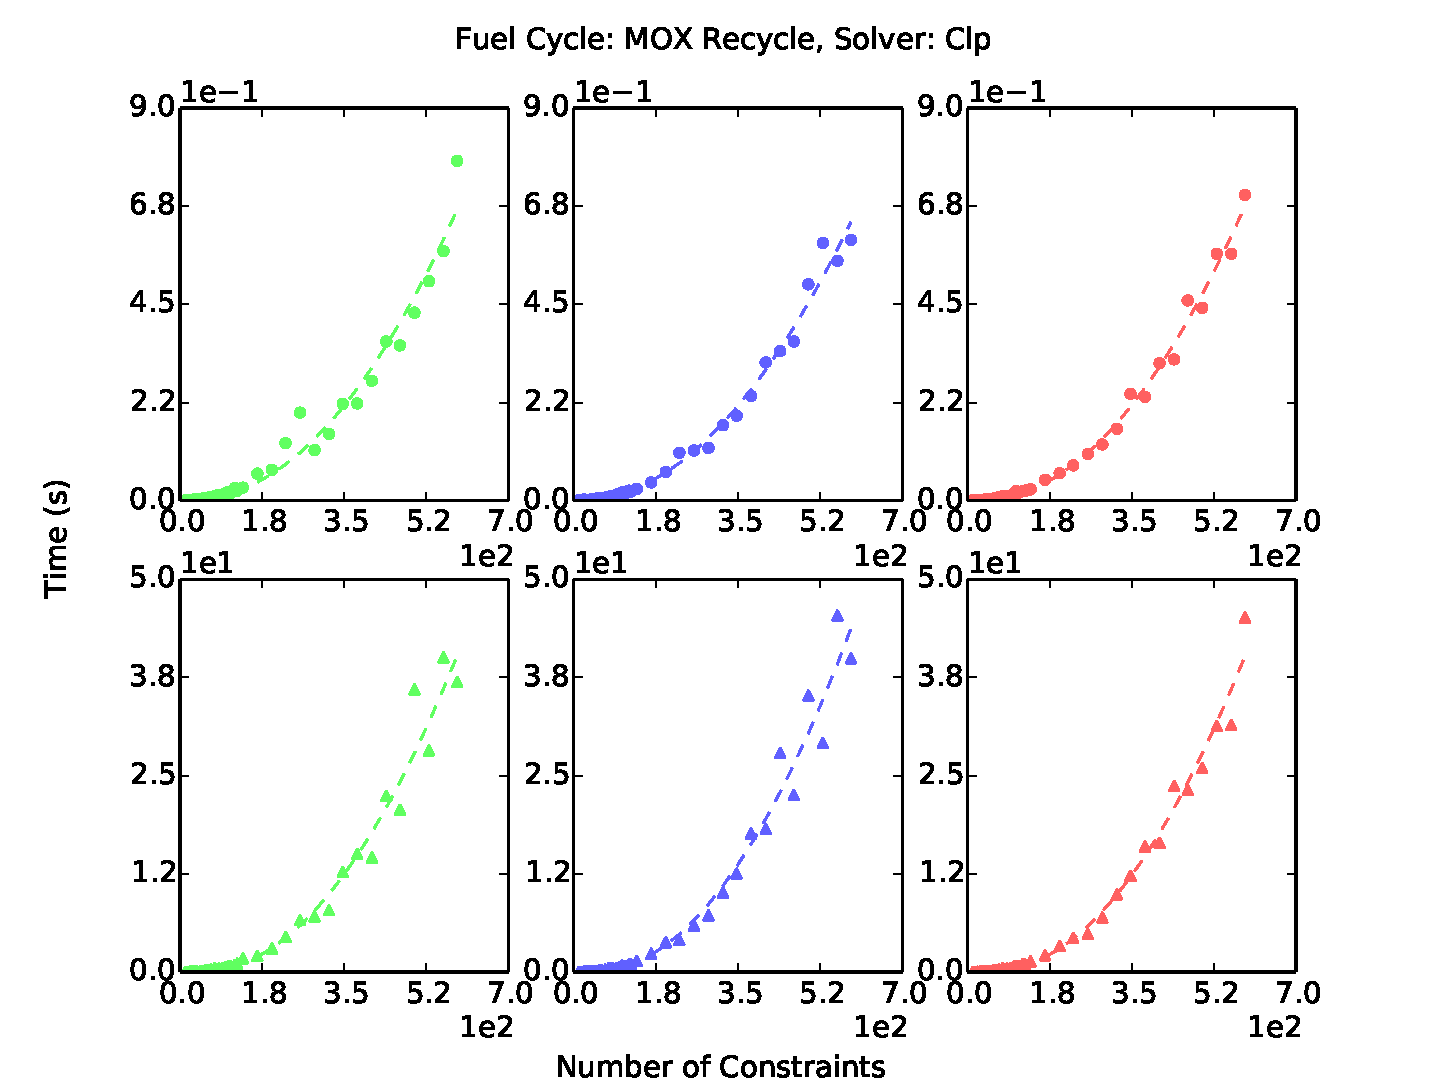
\includegraphics[width=.7\textwidth]{base_front_n_constrs_time_fc1_clp.pdf}
    \caption{
      \label{fig:base_front_n_constrs_time_fc1_clp}
      CLP Solver results for the MOX fuel cycle as the number of constraints
      increases.
      }
  \end{center}
\end{figure}

\begin{figure}[h!]
  \begin{center}
    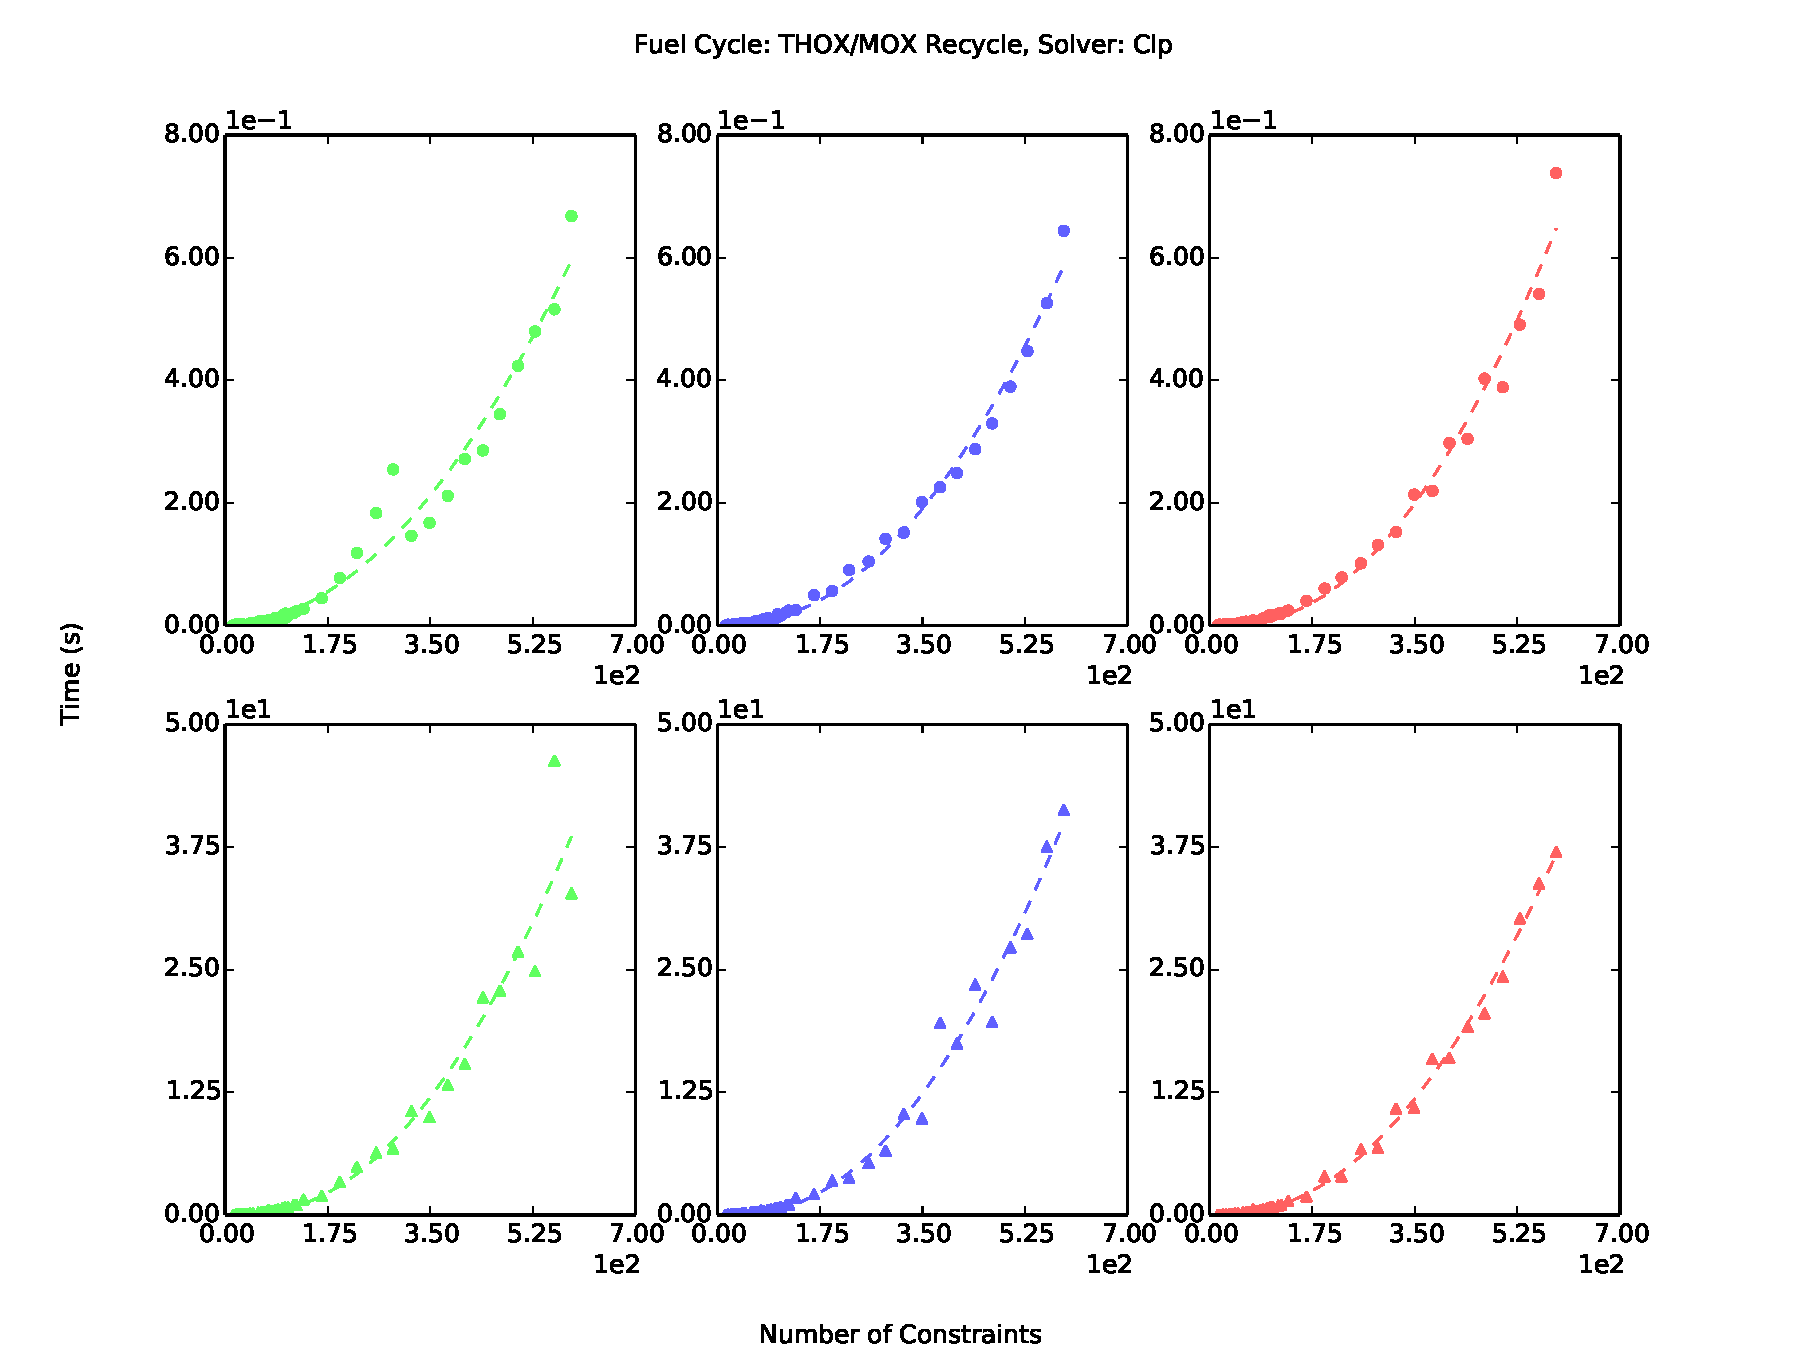
\includegraphics[width=.7\textwidth]{base_front_n_constrs_time_fc2_clp.pdf}
    \caption{
      \label{fig:base_front_n_constrs_time_fc2_clp}
      CLP Solver results for the ThOX fuel cycle as the number of constraints
      increases.
      }
  \end{center}
\end{figure}

\paragraph{\cbc Solver}

The performance of the \cbc solver is much more sporadic than either the CLP or
Greedy solvers. This is to be expected, for MILP optimization problems are
NP-Hard. Further, they are solved using enumeration techniques that do not
perform characteristically well, as the Simplex method does. 

\cbc was limited to 3 hours for each problem, and a 1\% ratio-gap convergence
criteria was applied. The term \textit{ratio gap} is in reference to the current
known upper and lower bound on the optimal objective value. During the
branch-and-bound algorithm, such bounds are maintained and updated between each
solution iteration (explained in more detail in Appendix \ref{app:ip}). The
solver reports an optimal solution when the criteria shown in Equation
\ref{eqn:ratio_gap} is true.

\begin{equation}\label{eqn:ratio_gap}
\frac{z_U - z_L}{z_U} \leq 0.01
\end{equation}

In each of the figures below, only instances reaching convergence are displayed
in order to attempt to ascertain any related
trends. \Cref{fig:base_front_n_rxtr_time_fc0_cbc,fig:base_front_n_rxtr_time_fc1_cbc,fig:base_front_n_rxtr_time_fc2_cbc}
show timing results as a function of the number of reactors in the
system. \Cref{fig:base_front_n_arcs_time_fc0_cbc,fig:base_front_n_arcs_time_fc1_cbc,fig:base_front_n_arcs_time_fc2_cbc}
show timing results as a function of the number of arcs in the system. Note that
in each case below, a log-linear graph is used. In each frame, the percentage of
converged instances is provided.

\begin{figure}[h!]
  \begin{center}
    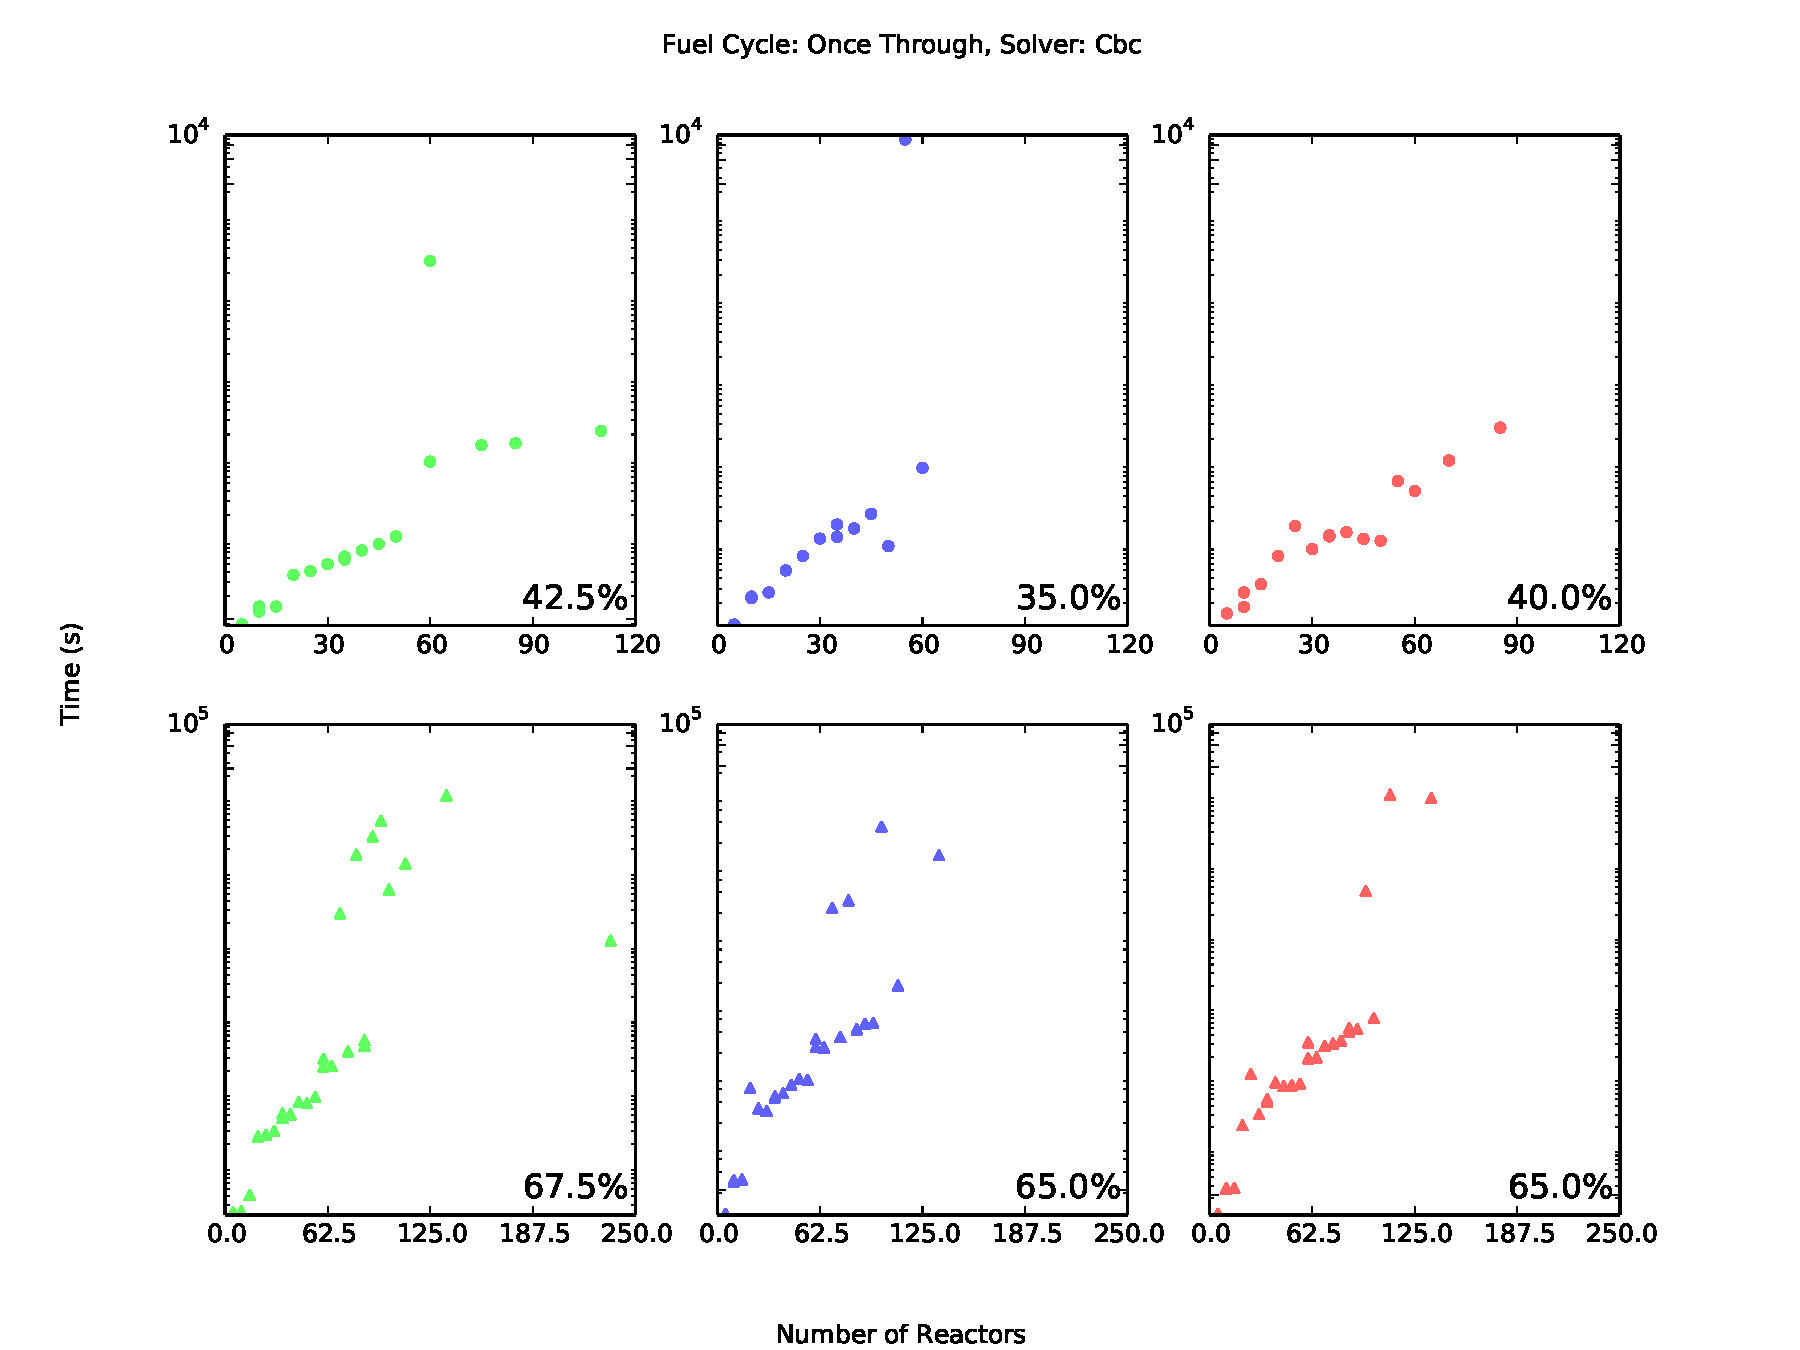
\includegraphics[width=.7\textwidth]{base_front_n_rxtr_time_fc0_cbc.pdf}
    \caption{
      \label{fig:base_front_n_rxtr_time_fc0_cbc}
      \cbc Solver results for the OT fuel cycle as the number of reactors
      increases.
      }
  \end{center}
\end{figure}

\begin{figure}[h!]
  \begin{center}
    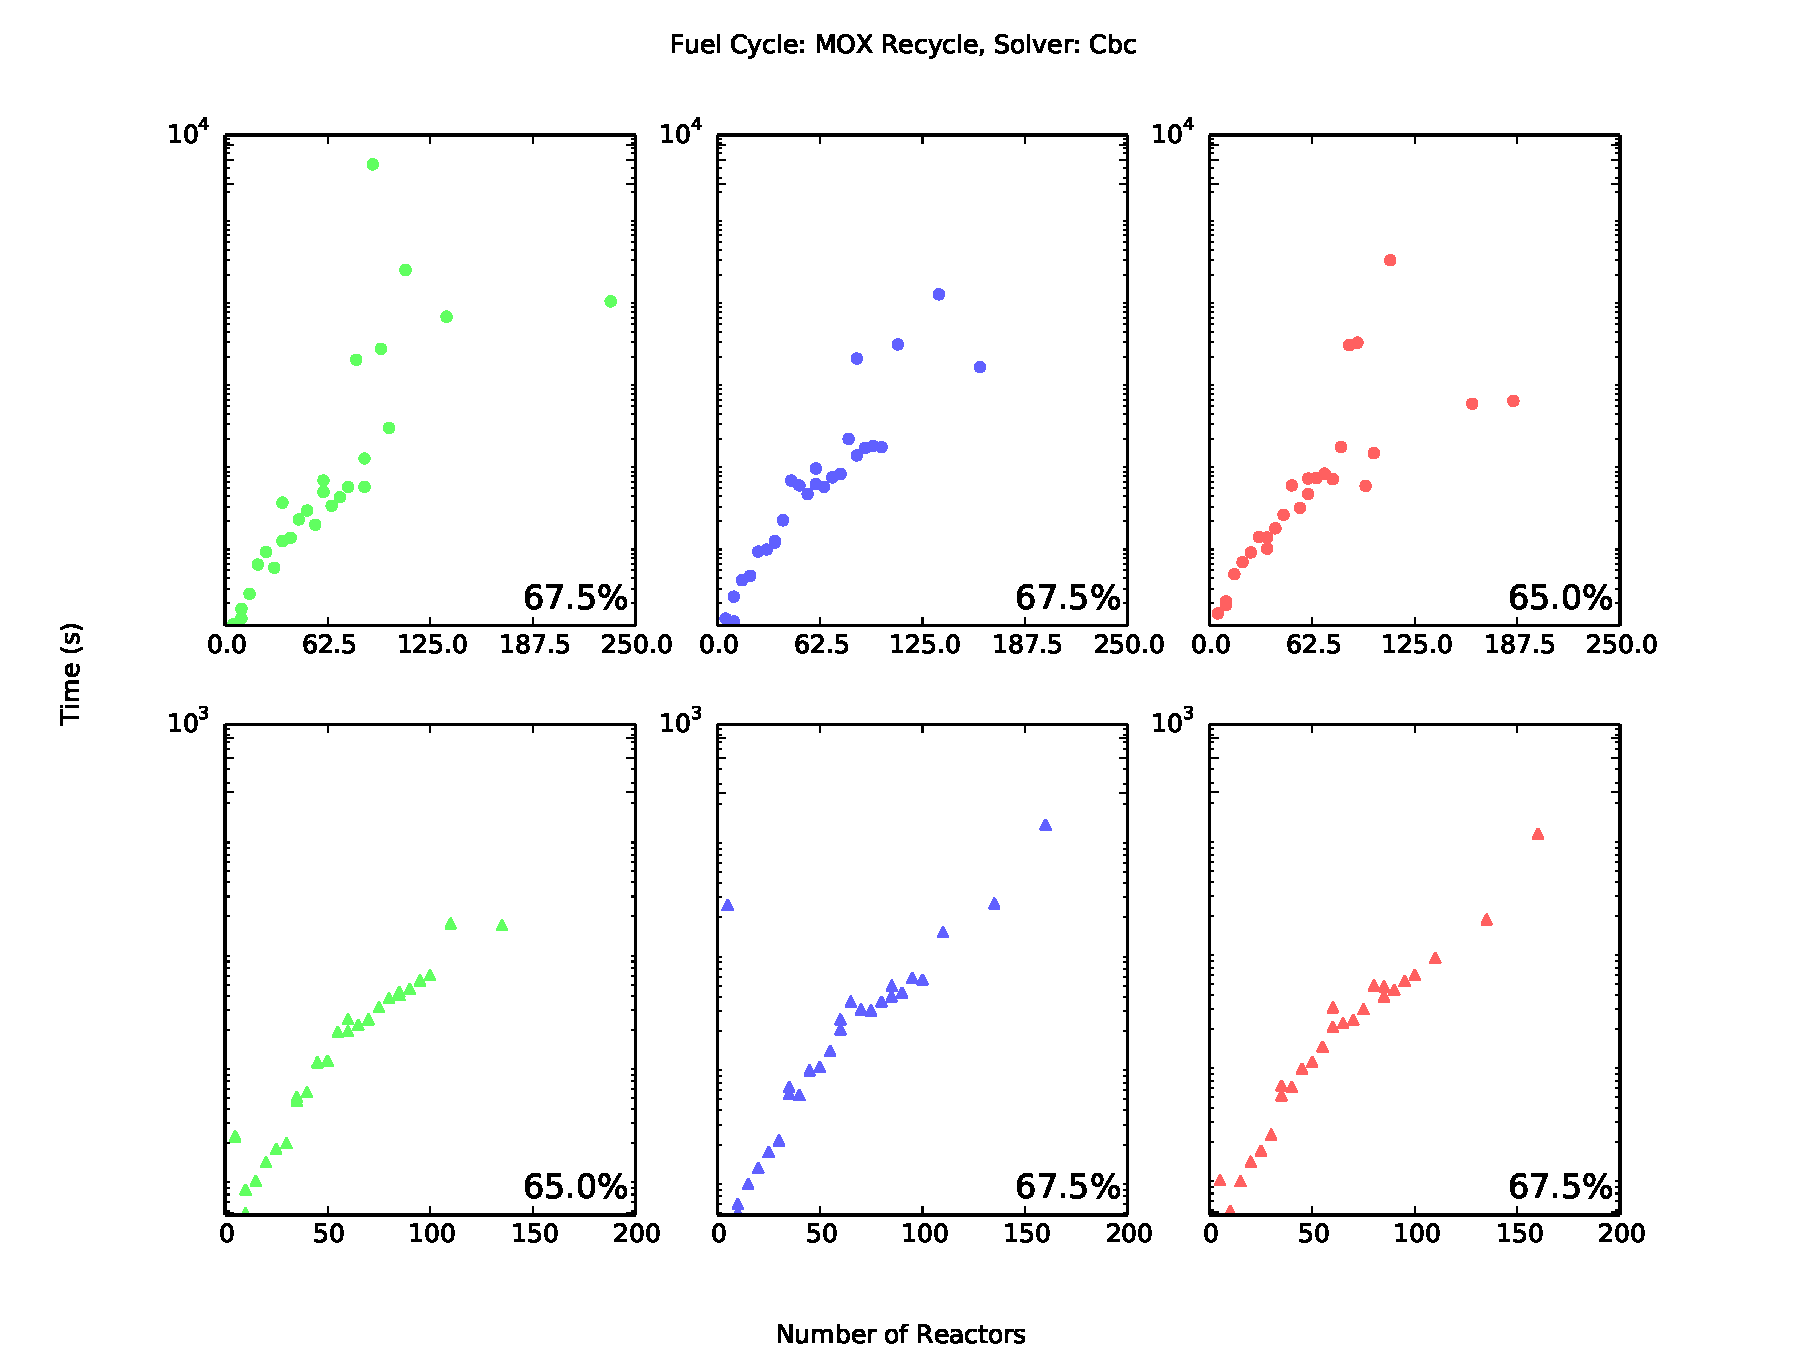
\includegraphics[width=.7\textwidth]{base_front_n_rxtr_time_fc1_cbc.pdf}
    \caption{
      \label{fig:base_front_n_rxtr_time_fc1_cbc}
      \cbc Solver results for the MOX fuel cycle as the number of reactors
      increases.
      }
  \end{center}
\end{figure}

\begin{figure}[h!]
  \begin{center}
    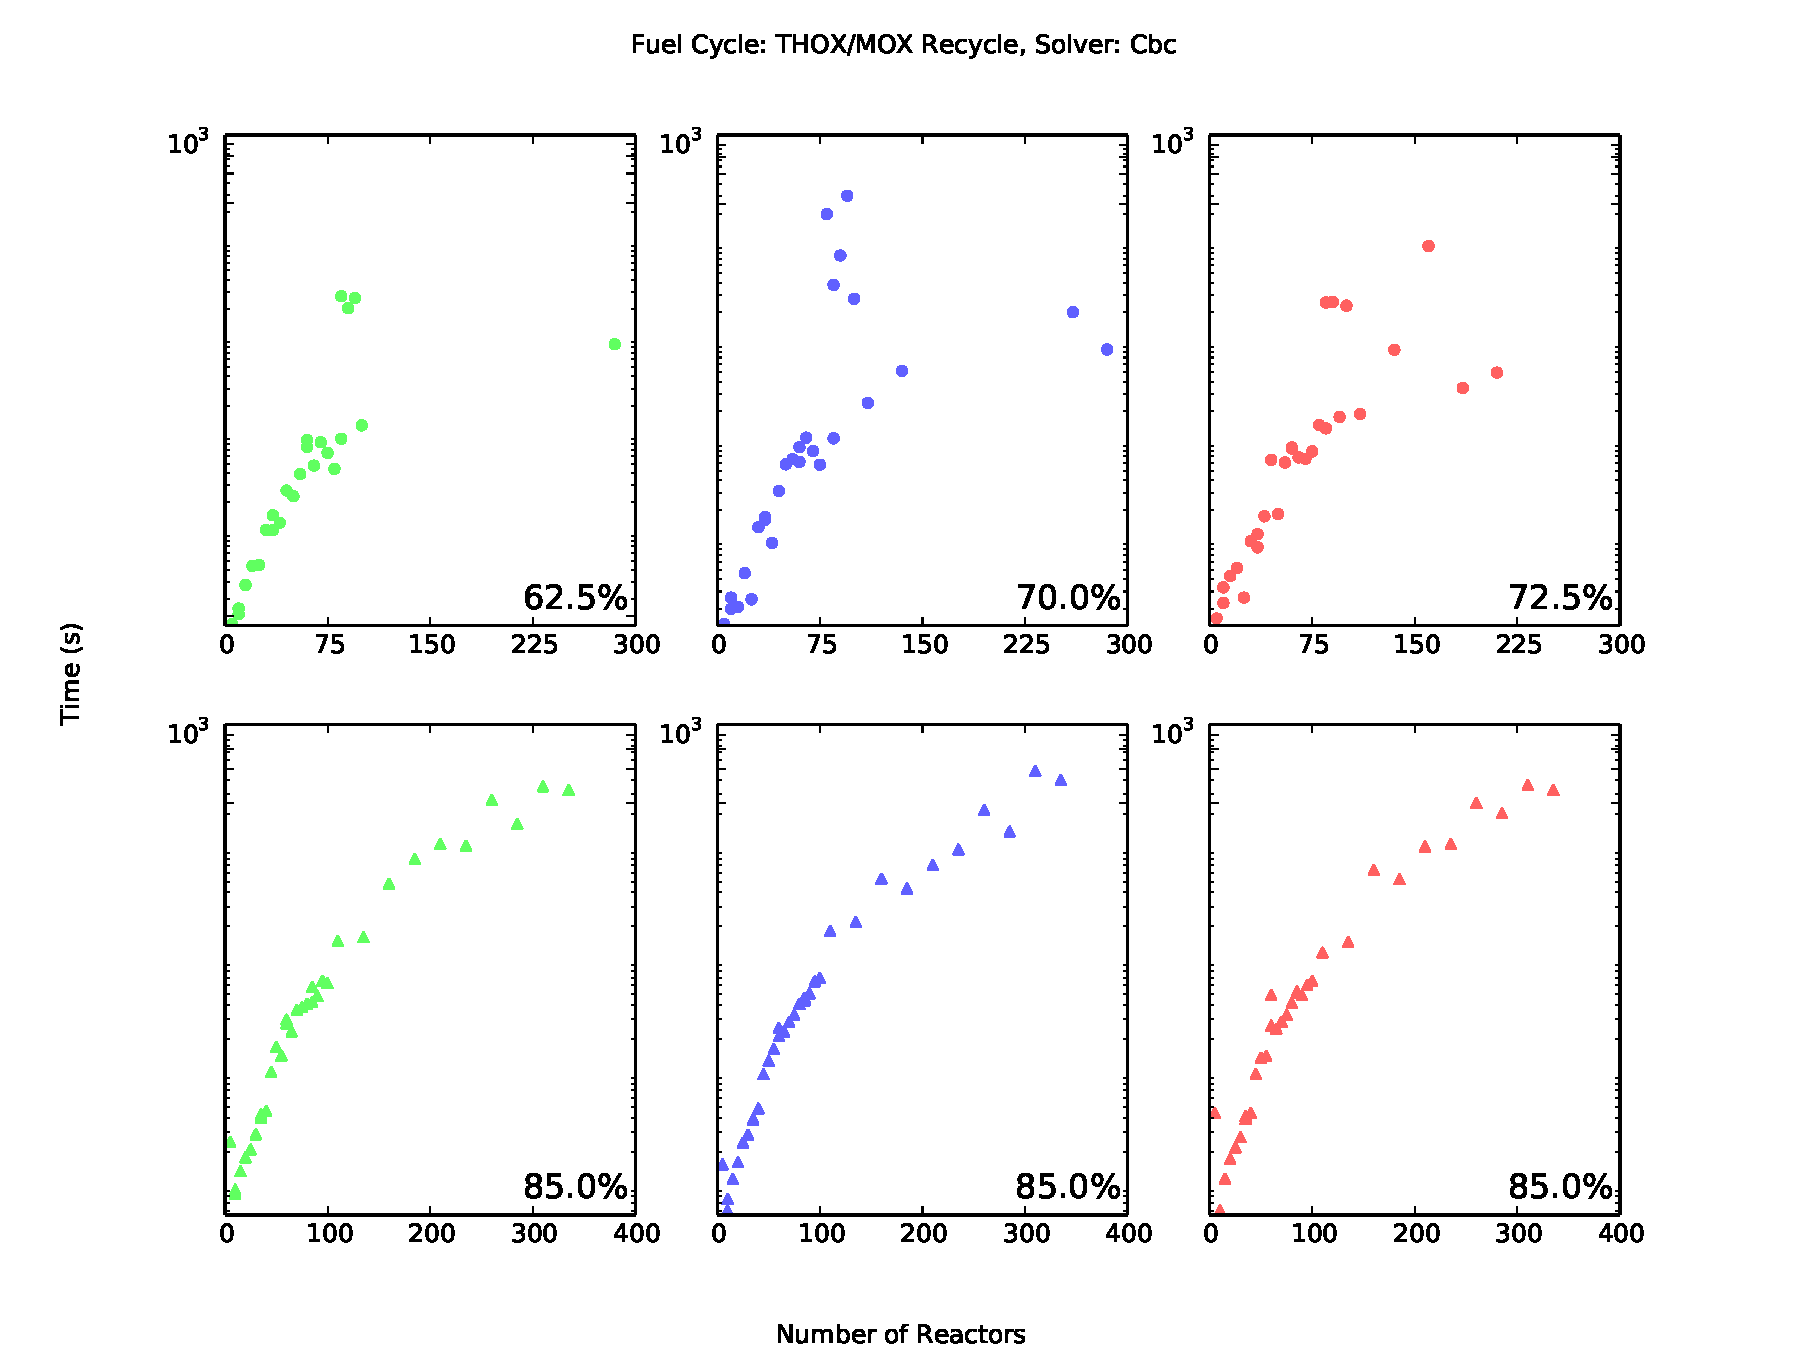
\includegraphics[width=.7\textwidth]{base_front_n_rxtr_time_fc2_cbc.pdf}
    \caption{
      \label{fig:base_front_n_rxtr_time_fc2_cbc}
      \cbc Solver results for the ThOX fuel cycle as the number of reactors
      increases.
      }
  \end{center}
\end{figure}

\begin{figure}[h!]
  \begin{center}
    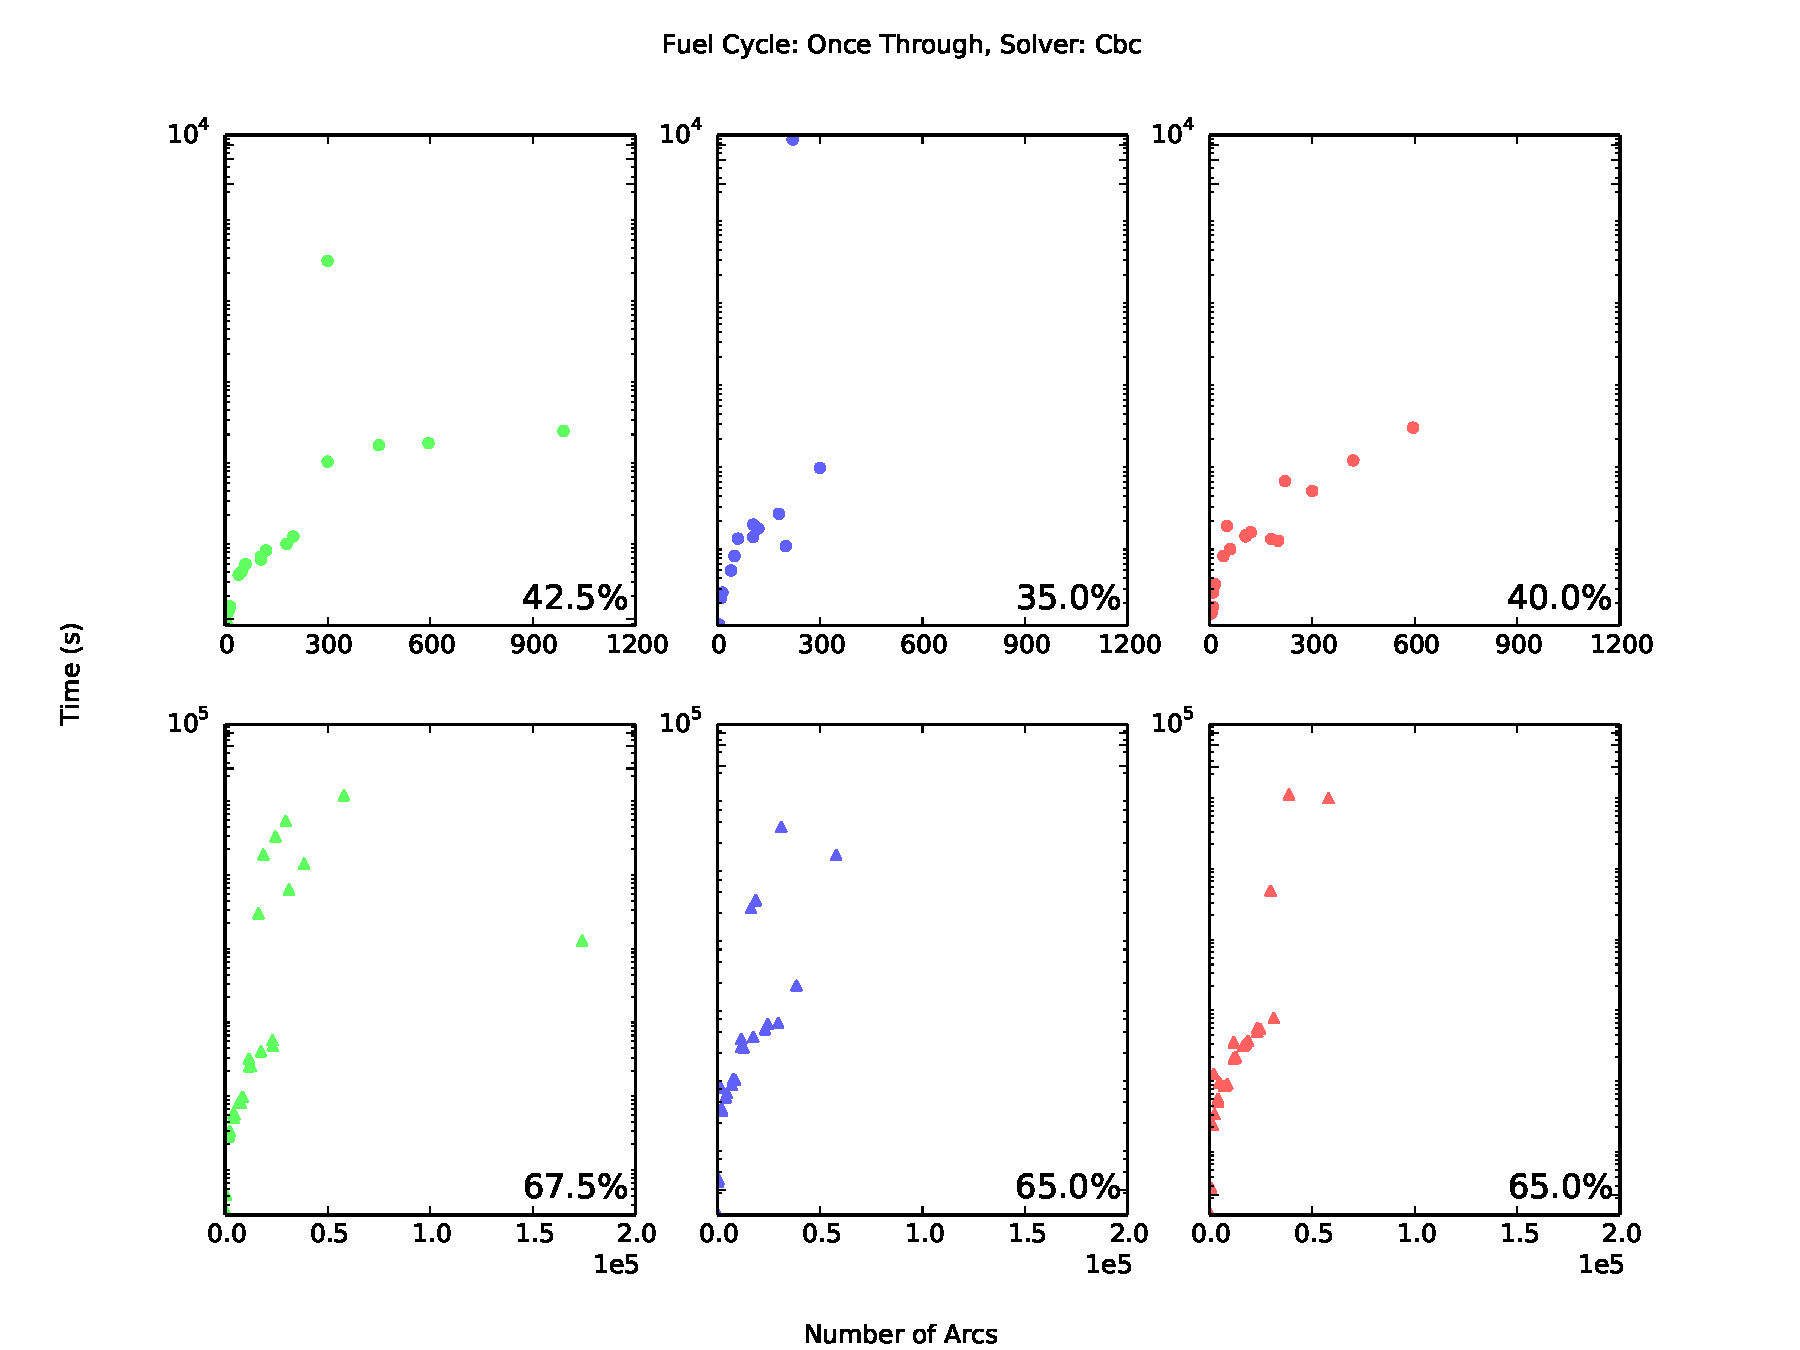
\includegraphics[width=.7\textwidth]{base_front_n_arcs_time_fc0_cbc.pdf}
    \caption{
      \label{fig:base_front_n_arcs_time_fc0_cbc}
      \cbc Solver results for the OT fuel cycle as the number of arcs
      increases.
      }
  \end{center}
\end{figure}

\begin{figure}[h!]
  \begin{center}
    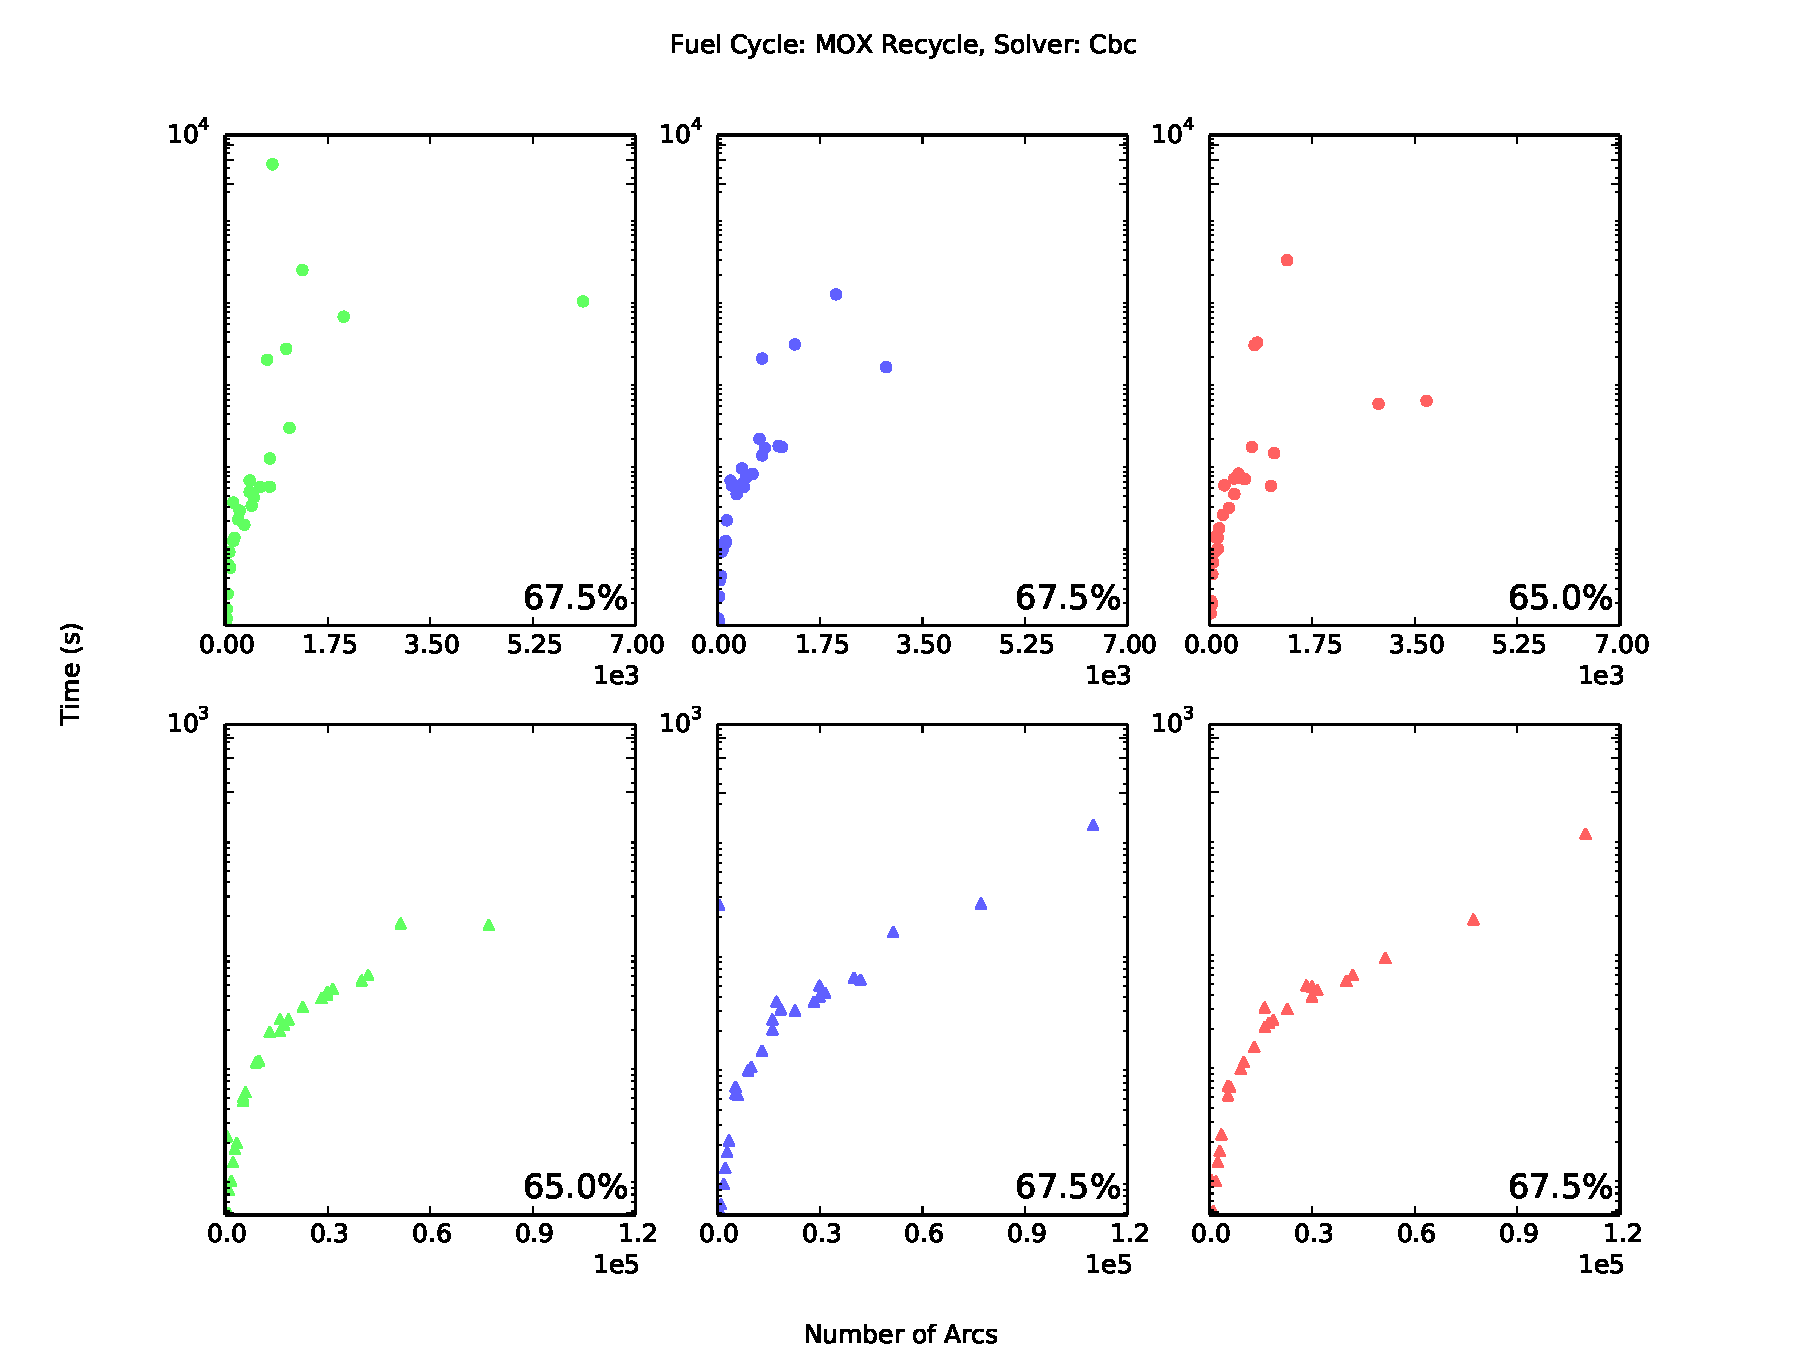
\includegraphics[width=.7\textwidth]{base_front_n_arcs_time_fc1_cbc.pdf}
    \caption{
      \label{fig:base_front_n_arcs_time_fc1_cbc}
      \cbc Solver results for the MOX fuel cycle as the number of arcs
      increases.
      }
  \end{center}
\end{figure}

\begin{figure}[h!]
  \begin{center}
    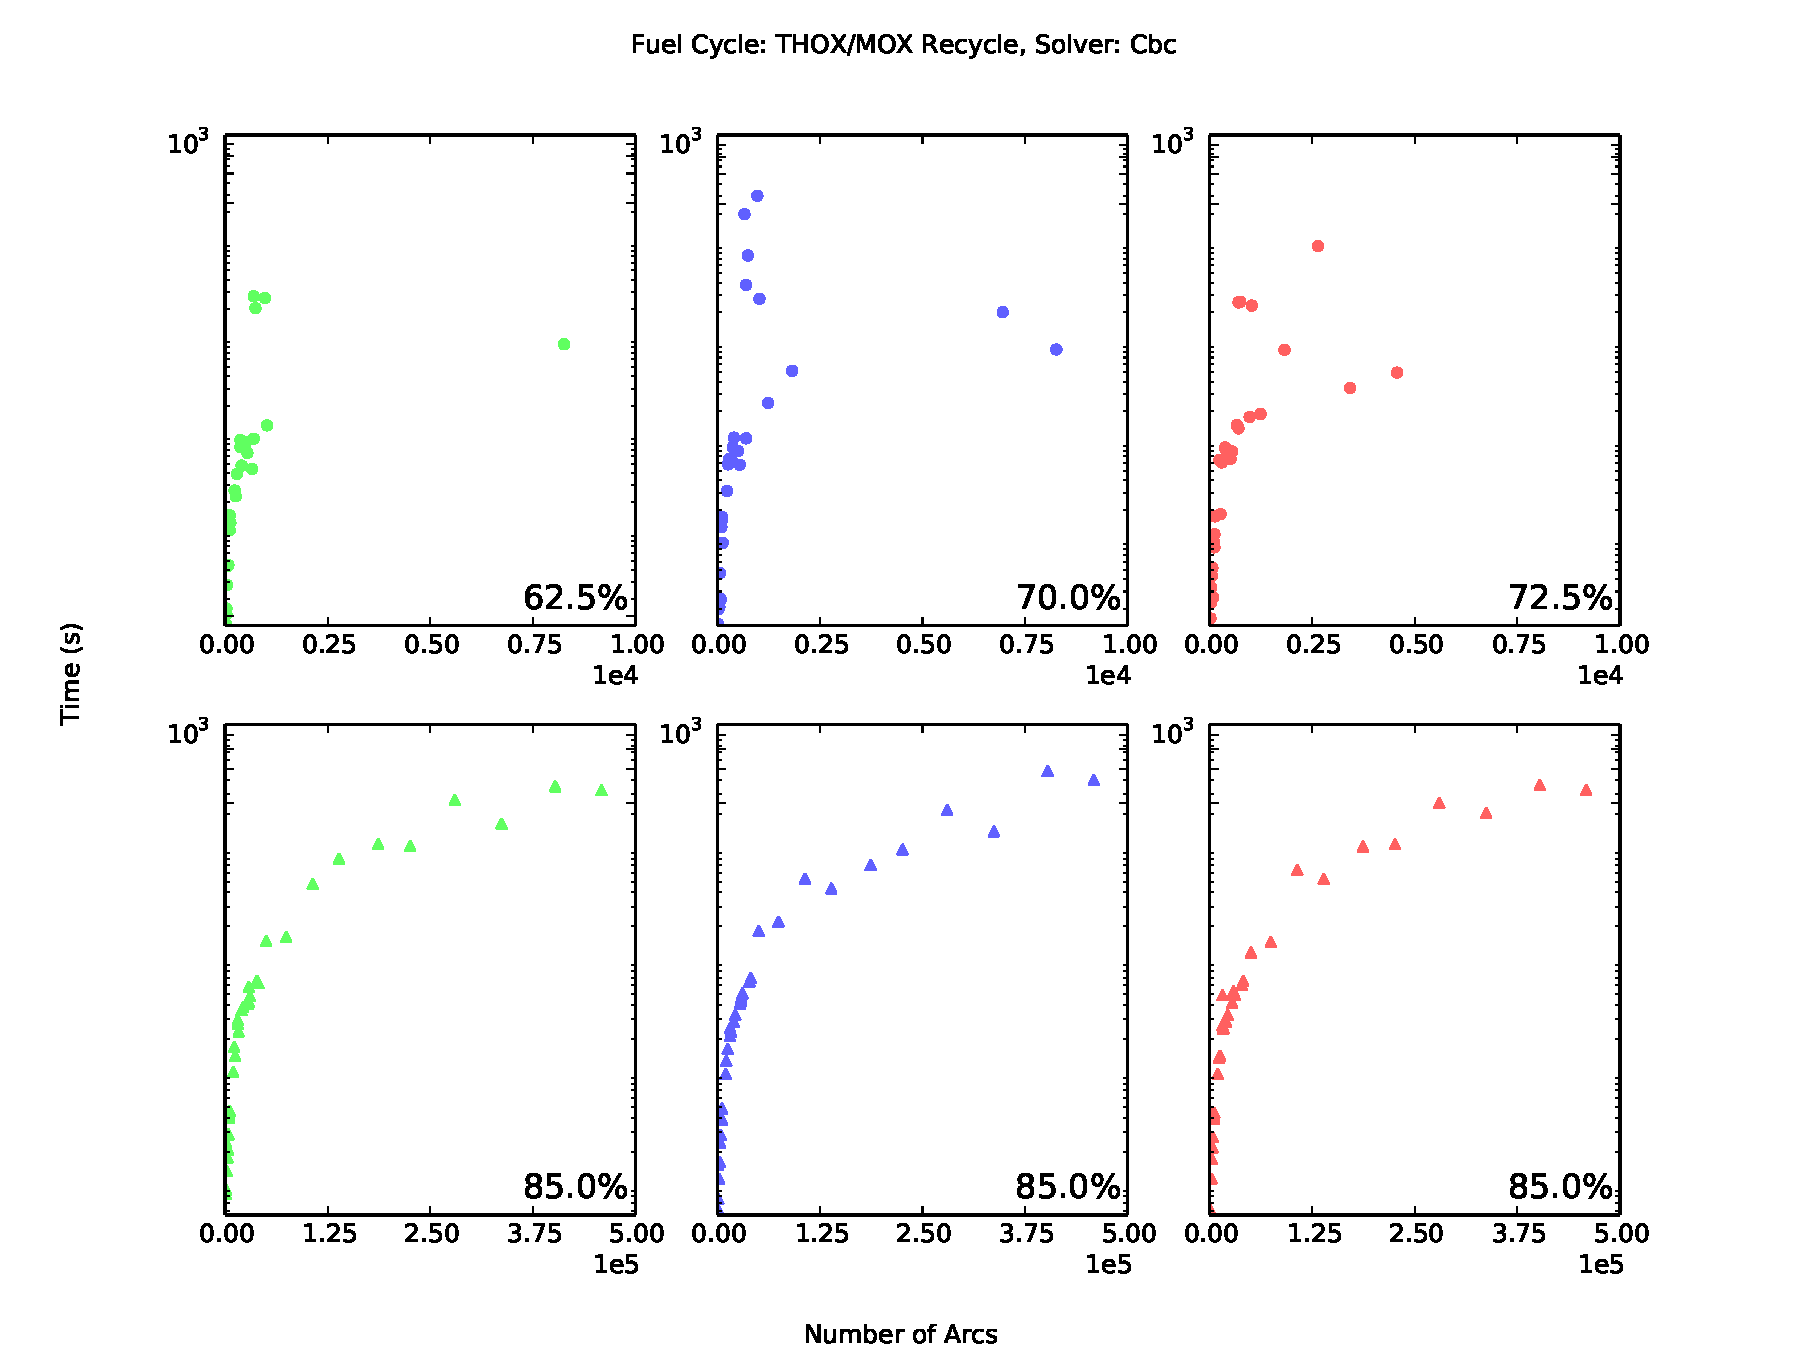
\includegraphics[width=.7\textwidth]{base_front_n_arcs_time_fc2_cbc.pdf}
    \caption{
      \label{fig:base_front_n_arcs_time_fc2_cbc}
      \cbc Solver results for the ThOX fuel cycle as the number of arcs
      increases.
      }
  \end{center}
\end{figure}

Immediately obvious, and slightly counter intuitive, is that the population of
converged instances is larger for assembly-based exchanges rather than
batch-based exchanges, even though the number of variables in the problem is
much lower for batch-based exchanges. Additionally, the \cbc solver converged in
many fewer instances for low reactor fidelity in the OT fuel cycle than either
MOX or ThOX cycles. Low-fidelity once-through cases have the least amount of
``choice'' in the system. There is a single commodity, consumer type, and
supplier type. Regardless of fuel cycle, reactor fidelity, or objective
coefficient strategy, the \cbc solver experiences exponential scaling with
problem size.

\subsubsection{Solution Comparison}\label{sec:res:scale:front:soln}

Solutions between any two solvers can be compared either in the formulation
layer or in the exchange layer. Comparison in the formulation layer is achieved
by comparing objective function values (Equation \ref{eqn:obj_flow}), whereas
comparison in the exchange layer is achieved by comparing a measure the flows
and preferences for a given solution (Equation \ref{eqn:sim_flow}). 

The objective function includes the costs and flows on false arcs which inflates
the objective function value. While the false arcs are necessary for
guaranteeing a feasible solution, their resulting flows are not taken into
account when the DRE back-translates from the formulation to the exchange
layer. Accordingly, $z^*_{\text{sim}}$ is used as the primary comparison
metric. While $z^* \leq z$ is true in cost space, $z^*_{\text{sim}} \geq
z_{\text{sim}}$ is \textit{not} necessarily true in practice for MILP
instances. Any MILP solver must use some convergence criteria, which takes into
account flow values along false arcs.

Comparisons are made between the Greedy solver and the \cbc solver, provided the
\cbc solver converged. A converged \cbc solution is guaranteed optimal within
the provided tolerance, and is therefore considered to be $z^*$ with a
corresponding set of flows $X^*$. Because solutions increase in magnitude with
increasing problem size, a relative comparison is made, as shown in Equation
\ref{eqn:sim_flow_compare}. The resulting features are similar across fuel
cycles. Accordingly, an example for the MOX fuel cycle is shown in Figure
\ref{fig:compare_cbc_greedy_pref_flow_front_n_rxtr__fc1_}.

\begin{equation}\label{eqn:sim_flow_compare}
\frac{z^*_{\text{sim}} - z_{\text{sim}, \text{Greedy}}}
     {z^*_{\text{sim}}} 
\end{equation}

\begin{figure}[h!]
  \begin{center}
    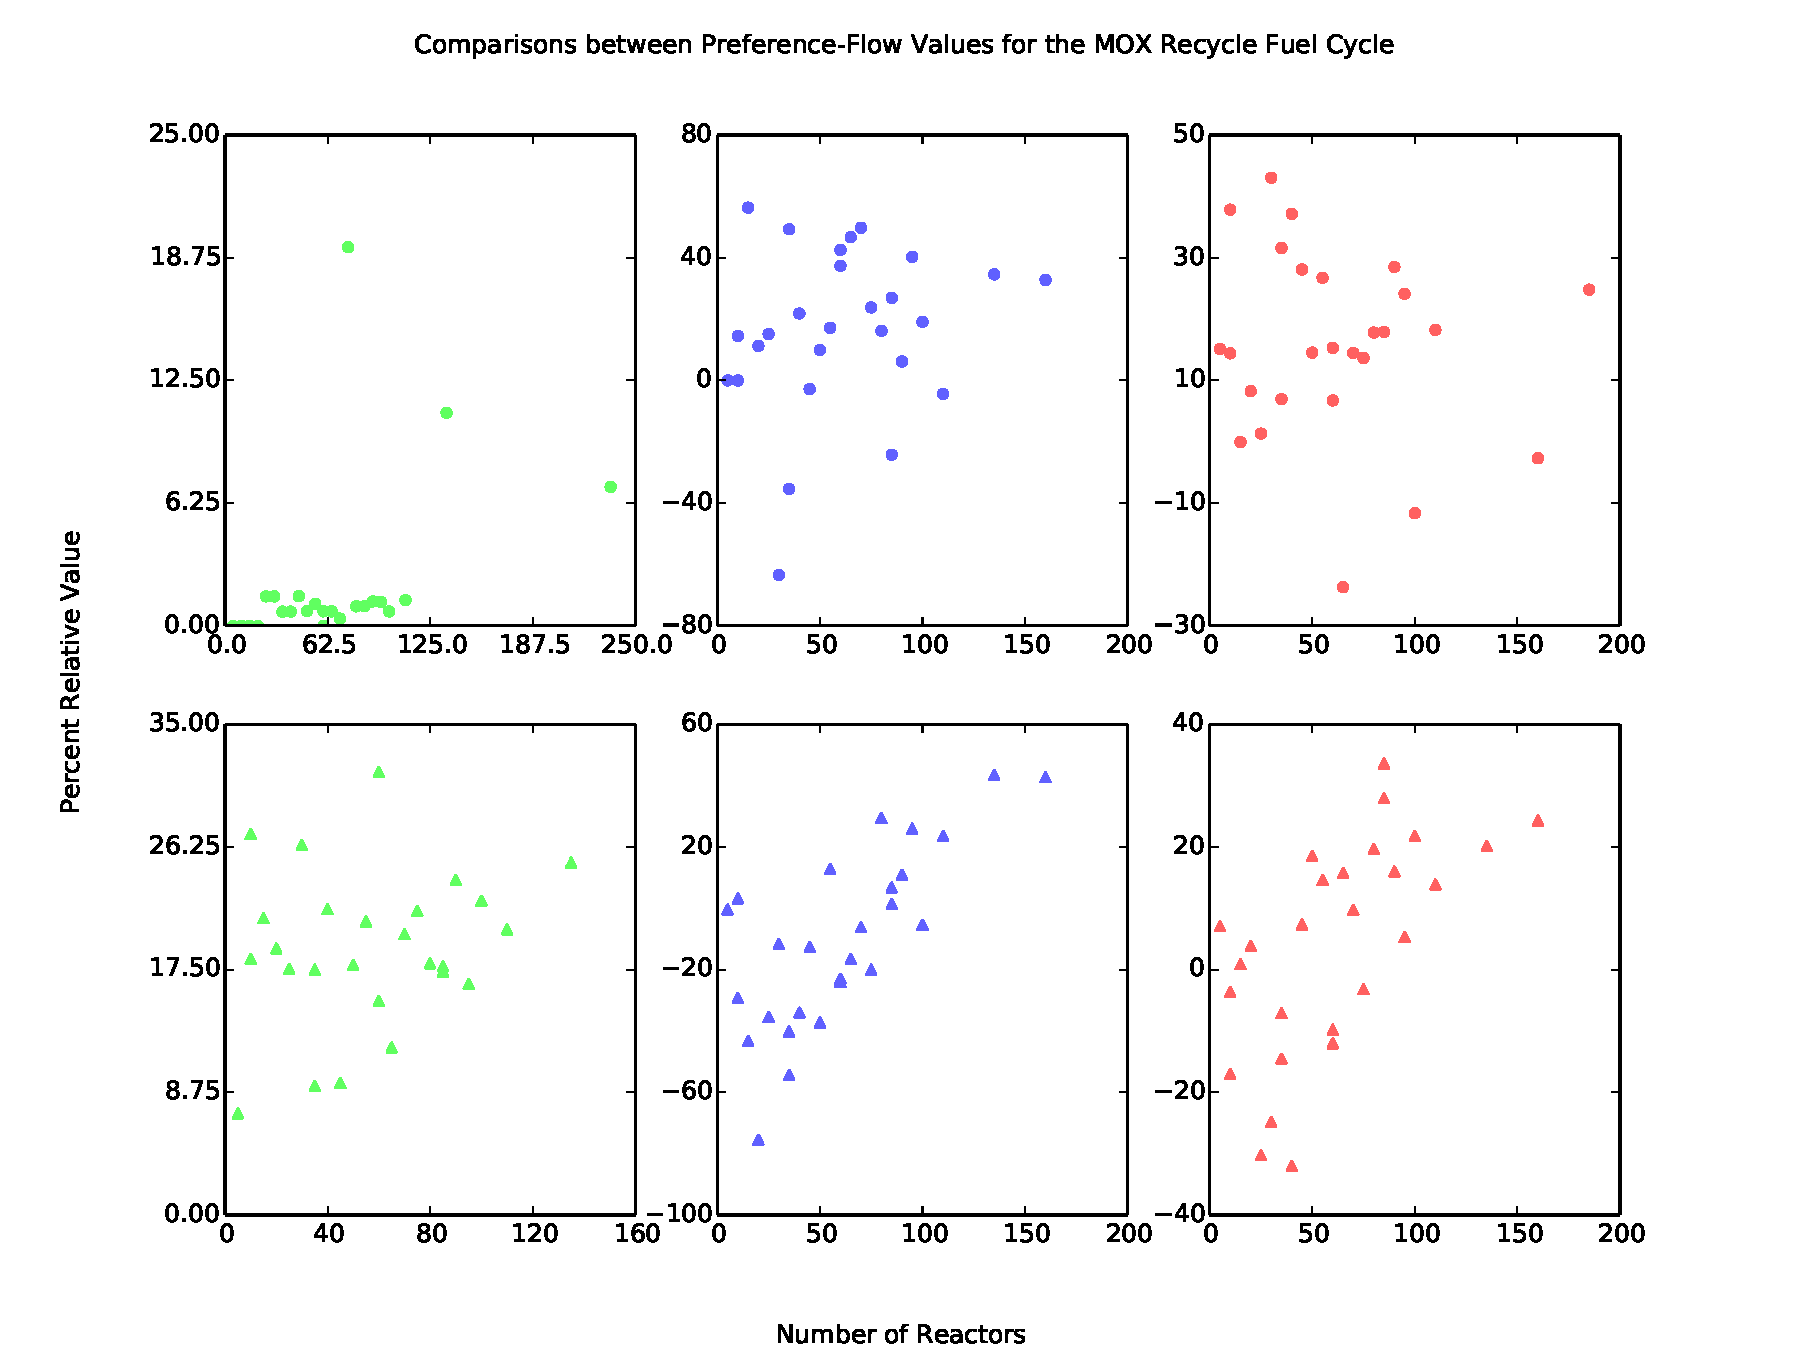
\includegraphics[width=.7\textwidth]{compare_cbc_greedy_pref_flow_front_n_rxtr__fc1_.pdf}
    \caption{
      \label{fig:compare_cbc_greedy_pref_flow_front_n_rxtr__fc1_}
      Comparisons between relative simulation metrics between the \cbc solver and
      the Greedy solver for MOX fuel cycles. Only converged \cbc
      solutions are compared.  }
  \end{center}
\end{figure}

Comparing the results in which there are no location-based preferences (green),
there is a clear correlation between the number of variables and the relative
benefit of using \cbc. The Greedy heuristic performs better when the number of
possible assignments is small. This is not unexpected; as the number of decision
variables increases, making optimial decisions should, in theory, result in a
increasingly better outcomes than making heuristic-based decisions. 

Two features of interest arise when comparing the cases in which there is a
coarse location preference (blue) and a fine location preference (red). First,
some values are negative, implying that the Greedy solver provides a better
preference-space solution than the \cbc solver. Importantly, this is true only
in preference space; the \cbc always performs better in cost space, by
definition. The Greedy solver is allowed to provide better answers in preference
space for two reasons: the problem is highly constrained, and false arcs have an
arbitrarily high unit cost. \cbc converges when the criteria in Equation
\ref{eqn:ratio_gap} is met. When a problem is highly constrained, many false
arcs will be activated, contributing a large amount to the objective
function. If the choice between two possible flows is sufficiently small, i.e.,
small relative to $z^*$, then either solution may be returned upon convergence
depending on the branch-and-bound search path. Thus, good solutions in
preference-space are somewhat lost in the ``noise'' of cost-space.

%TODO: make sure to address 125-1
Second, this effect is reduced when the objective choice in cost-space increase,
as shown in case of fine location preference. In other words, the relative
benefit of using a heuristic over a full \cbc solve in preference space for the
problems run above appears to be a function of the size of \textit{possible}
objective coefficient values. Furthermore, the effect of objective coefficient
population size decreases as problem size increases. However, as can be seen
from Figure \ref{fig:compare_cbc_greedy_pref_flow_front_n_rxtr__fc1_}, this
benefit requres a relatively large, high-fidelity reactor simulation, i.e., more
than $\sim$80 reactors, to be consistently observed. 

This behvaior is more pronounced as the number of possible connections
increases. Consider the ThOX fuel-cycle results shown in Figure
\ref{fig:compare_cbc_greedy_pref_flow_front_n_rxtr__fc2_}. Again, large
variations are observed for instances with some location preference with small
reactor populations, especially for high-fidelity reactor instances. However, as
the reactor populations increase, \cbc solutions appear to asymptototically
appraoch relative values close to the base line set by simulations in which
there are no location-based preferences.

\begin{figure}[h!]
  \begin{center}
    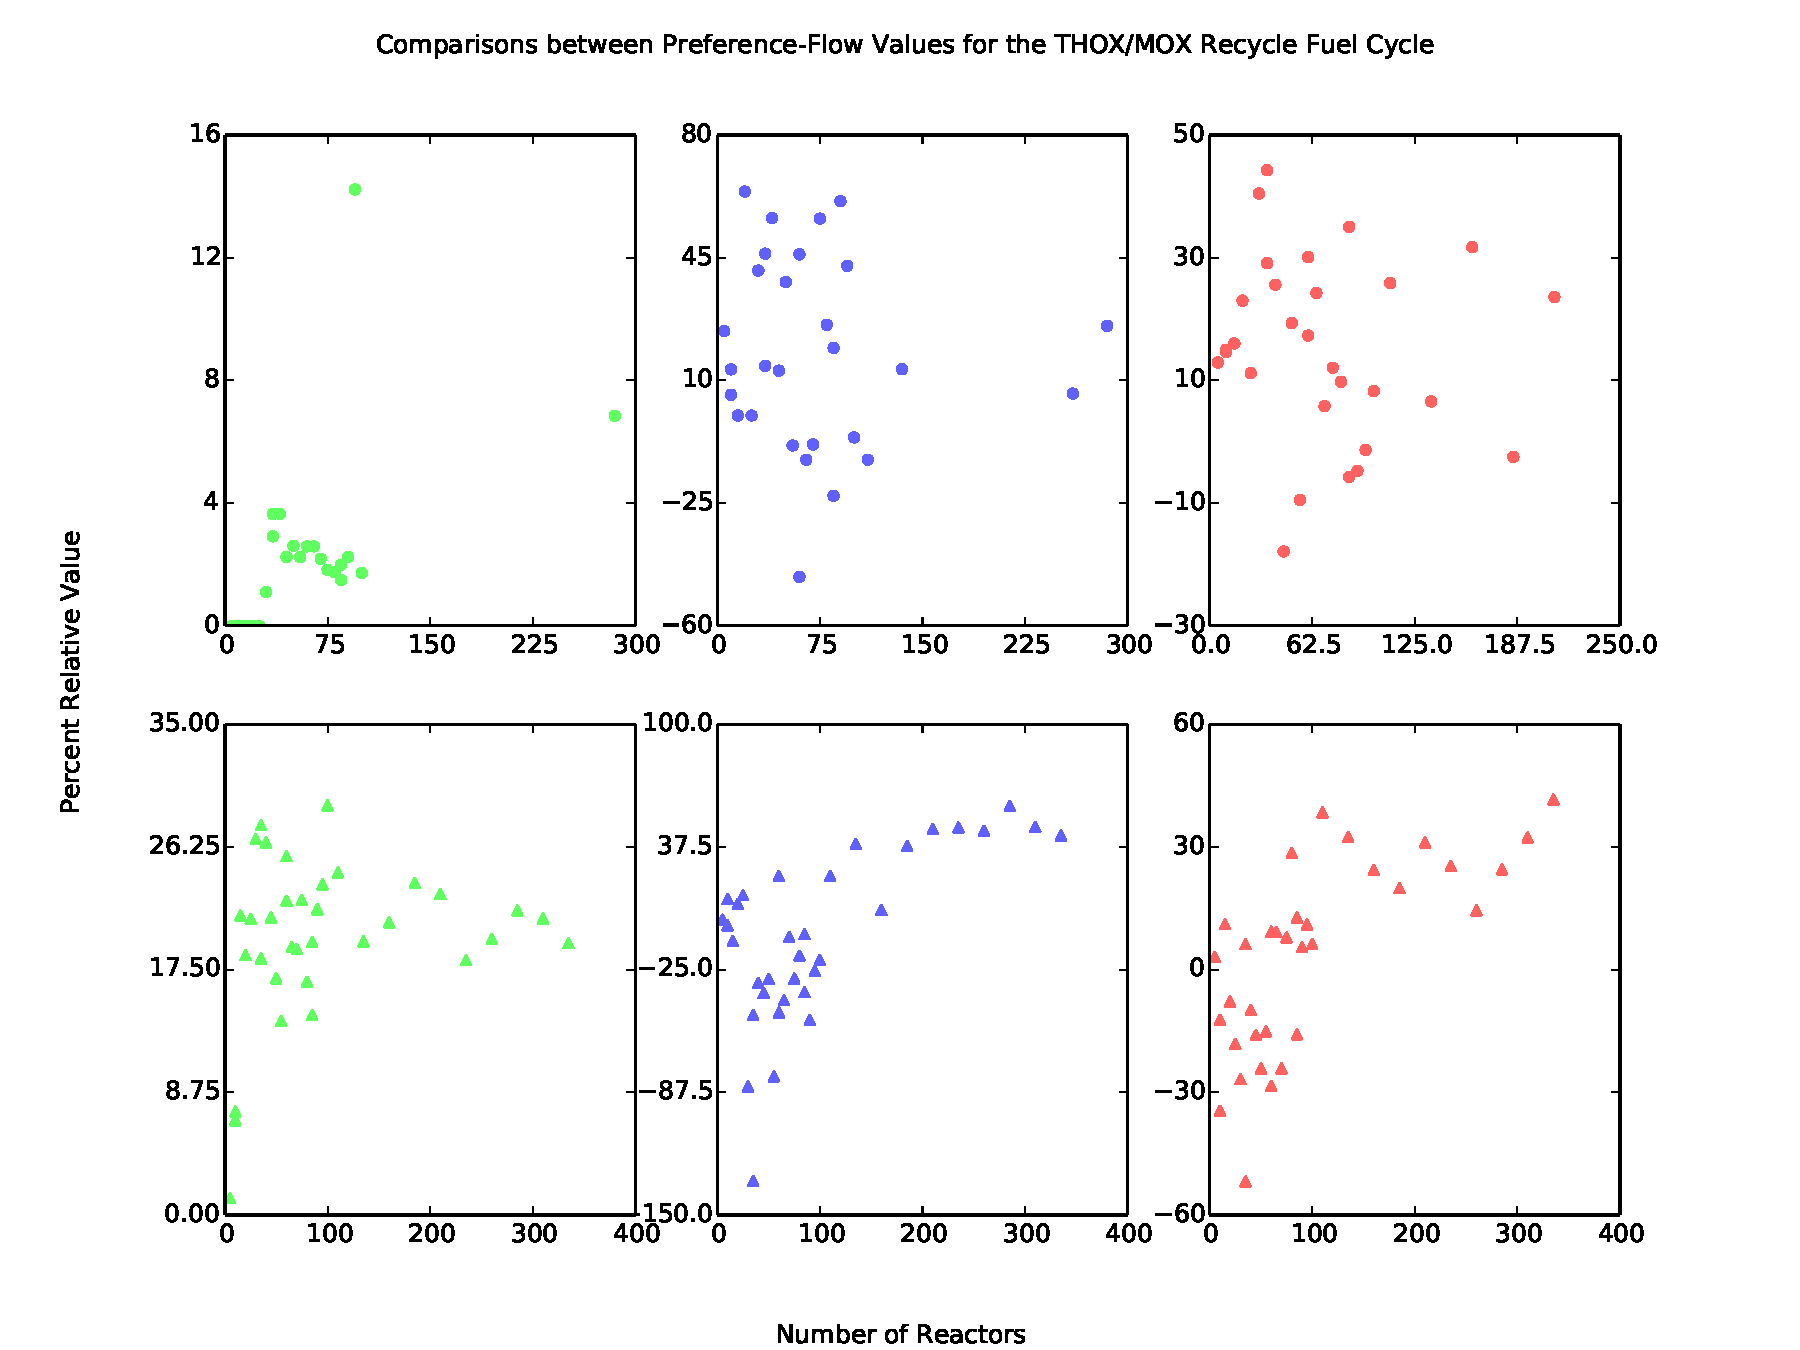
\includegraphics[width=.7\textwidth]{compare_cbc_greedy_pref_flow_front_n_rxtr__fc2_.pdf}
    \caption{
      \label{fig:compare_cbc_greedy_pref_flow_front_n_rxtr__fc2_}
      Comparisons between relative simulation metrics between the \cbc solver and
      the Greedy solver for ThOX fuel cycles. Only converged \cbc
      solutions are compared.  }
  \end{center}
\end{figure}

The Greedy solver can provide quite good preference-space results relative to
the \cbc solver when an exchange is highly constrained \textit{and} when the cost
coefficient assigned to false arcs is relatively large. This effect can be
observed by adjusting the false-arc cost coefficient, e.g., as shown in Equation
\ref{eqn:small_false_cost}. Two exchanges for which the Greedy solver performed
better in preference-space were chosen to demonstrate the effect. The results
are shown in Table \ref{tbl:false_arcs}. Note that it every case, $z$ is smaller
for the Greedy solver than \cbc; however, $z_\text{sim}$ for the Greedy solver is
larger than the same value with a large \cbc false-arc cost and smaller than
values related to small \cbc false-arc costs.

\begin{equation}\label{eqn:small_false_cost}
c_\text{false} = \frac{1}{p_\text{max}} + 1
\end{equation}

\begin{table}[h!]
\centering
\caption{Results from Reducing False-Arc Cost Coefficients.}
\label{tbl:false_arcs}
\begin{tabular}{|c|c|c|c|c|c|c|}
\hline
\multirow{2}{*}{\textbf{Simulation ID}} 
& \multicolumn{2}{c|}{\textbf{Greedy}} 
& \multicolumn{2}{c|}{\textbf{\cbc, Large Cost}} 
& \multicolumn{2}{c|}{\textbf{\cbc, Small Cost}} \\ \cline{2-7} 
& $z$ (large/small)        & $z_{\text{sim}}$        
& $z$             & $z_{\text{sim}}$            
& $z$             & $z_{\text{sim}}$            \\ \hline
54a5a92ce1ad43e9a713abf114b58a06
& 5.2e8/1.9e6 & 1.41e5
& 5.0e8 & 1.38e5
& 1.8e6 & 1.98e5 \\ \hline
938d808a4bd84346b54f38fcb4992386
& 3.97e8/1.40e6 & 1.08e5
& 3.81e8 & 8.8e4
& 1.38e6 & 1.12e5 \\ \hline
\end{tabular}
\end{table}

\subsubsection{Convergence Criteria}

The \cbc solver is highly tuneable. As with many iterative solution techniques,
the most critical tuneable criteria affecting the balance between solution
quality and solution time is the convergence criteria. It is not clear to what
degree solution quality will matter for users of Cyclus. Accordingly, a short
exploratory experiment was conducted to examine to what degree convergence
criteria affects solution time.

\cbc uses either an absolute or relative upper and lower-bound gap tolerance as
possible convergence criteria. All results discussed use the relative gap,
termed \textit{ratio gap} in \cbc parlance, as shown in Equation
\ref{eqn:ratio_gap}. For each of the 18 combinations of fundamental parameters,
10 instances of exchanges were executed, spanning a reactor population range of
10 to 500. Figure \ref{fig:hist_front_rxtr_0} displays the results for runs with
reactors trading full batches for ratio gap values of 0.1, 1, and 10\%. Figure
\ref{fig:hist_front_rxtr_1} displays the results for runs with reactors trading
individual assemblies for ratio gap values of 1 and 10\%.

\begin{figure}[h!]
  \begin{center}
    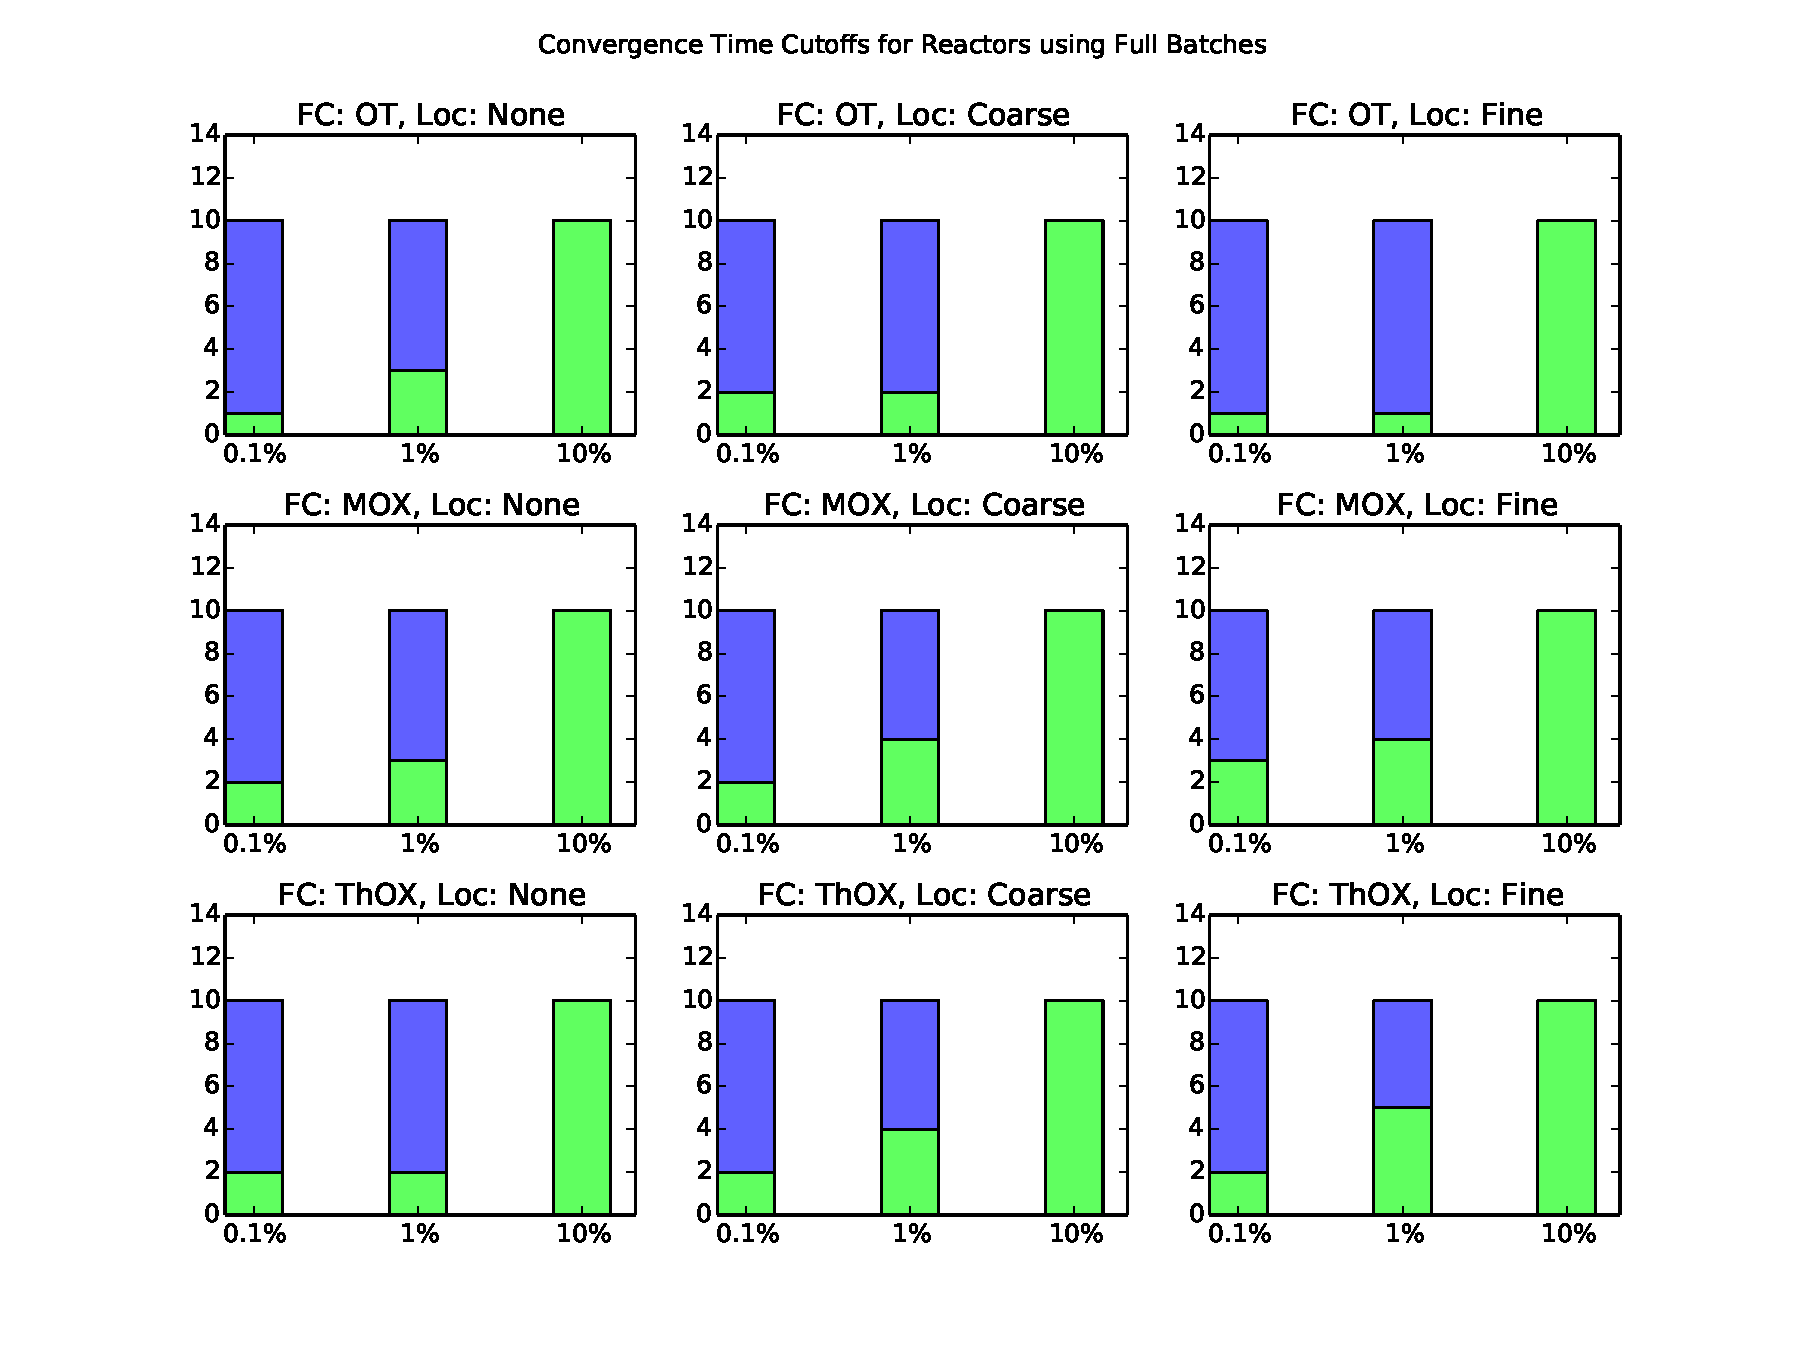
\includegraphics[width=.95\textwidth]{hist_front_rxtr_0.pdf}
    \caption{
      \label{fig:hist_front_rxtr_0}
      Effects of increasing convergence criteria on Front-End exchanges with
      reactors exchanging batches. Each bar is divided into how many instances
      converged (green) and did not converge (blue). }
  \end{center}
\end{figure}

\begin{figure}[h!]
  \begin{center}
    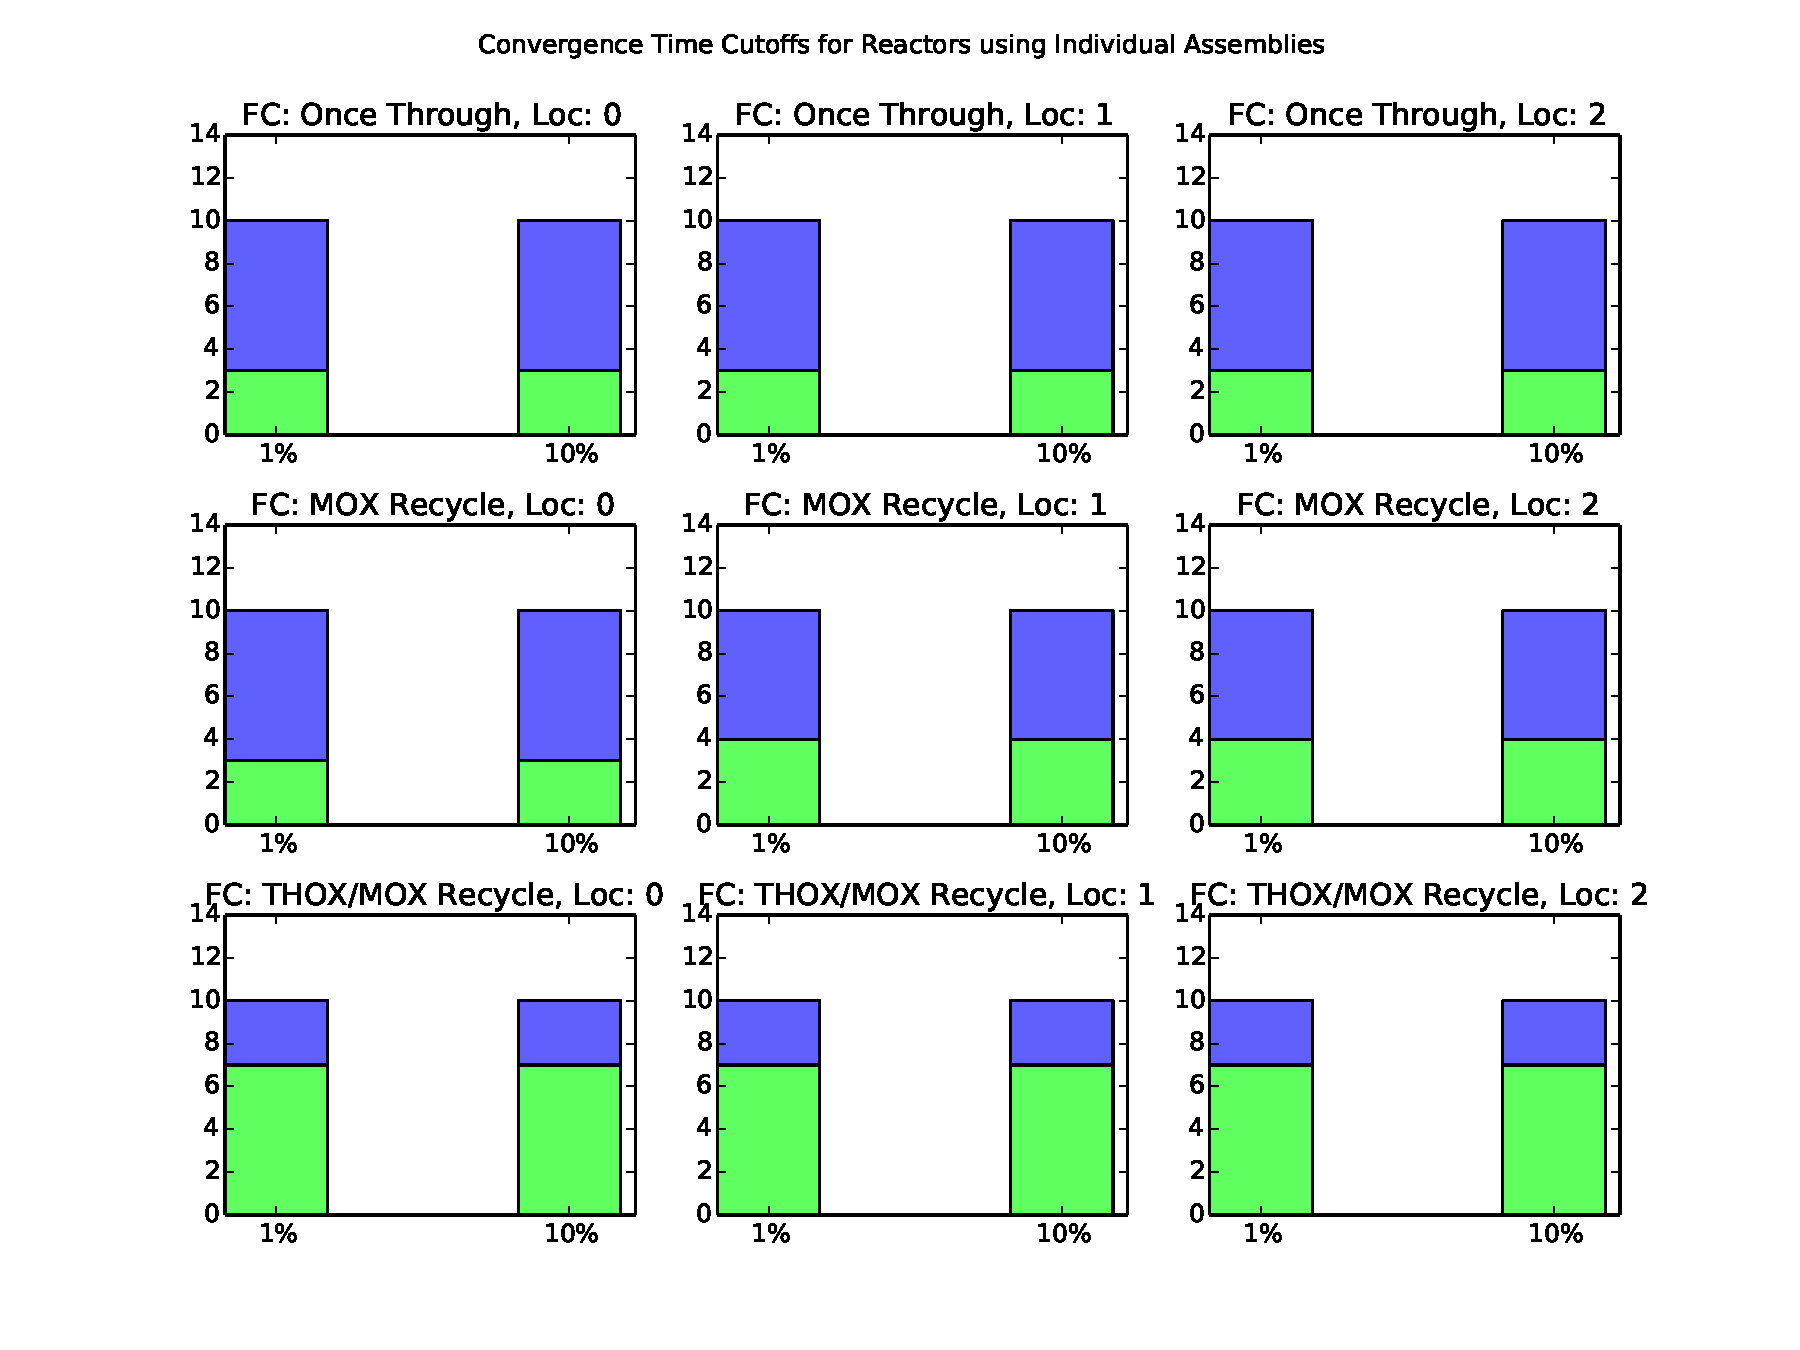
\includegraphics[width=.95\textwidth]{hist_front_rxtr_1.pdf}
    \caption{
      \label{fig:hist_front_rxtr_1}
      Effects of increasing convergence criteria on Front-End exchanges with
      reactors exchanging assemblies. Each bar is divided into how many instances
      converged (green) and did not converge (blue).}
  \end{center}
\end{figure}

Increasing the convergence criteria for smaller problems, i.e., those with
reactors requesting a single batch of fuel, has a greater effect than increasing
the convergence criteria for larger problems. It is somewhat surprising that the
increase from a 1\% relative bound gap to a 10\% gap allows full convergence in
the smaller case and has no effect in the larger case. Considering the
discussion in \secref{sec:res:scale:front:soln}, it is likely that the large
convergence effect is due increasing the ``noise'' effect of actual
arcs. However, some speed ups in solution times are expected when relaxing
convergence criteria, and those speed ups will likely be more profound in
smaller-sized problems than larger problems based on this analysis.

\subsection{Back-End Exchanges}

Many of the results of the back-end exchanges mirror those of the front-end
exchanges. Therefore, this section will discuss only differences between the two
cases. The fact that so many similarities exist is somewhat striking, because
from a simulation perspective, back-end exchanges are quite different than
front-end exchanges. First, a single request is made for each commodity type
that can be consumed by support facilities. Therefore, many fewer requests exist
in the system. Next, the supply of used fuel is known. A new supporting facility
type, repositories, are also added, resulting in a slightly higher total arc
population per reactor. As with the front-end exchanges, the arc population
scales as $\mathcal{O}(n^2)$, as can be seen in Figure
\ref{fig:base_back_n_rxtr_n_arcs_fc1_greedy}, and the constraint population
scales as $\mathcal{O}(n)$.

\begin{figure}[h!]
  \begin{center}
    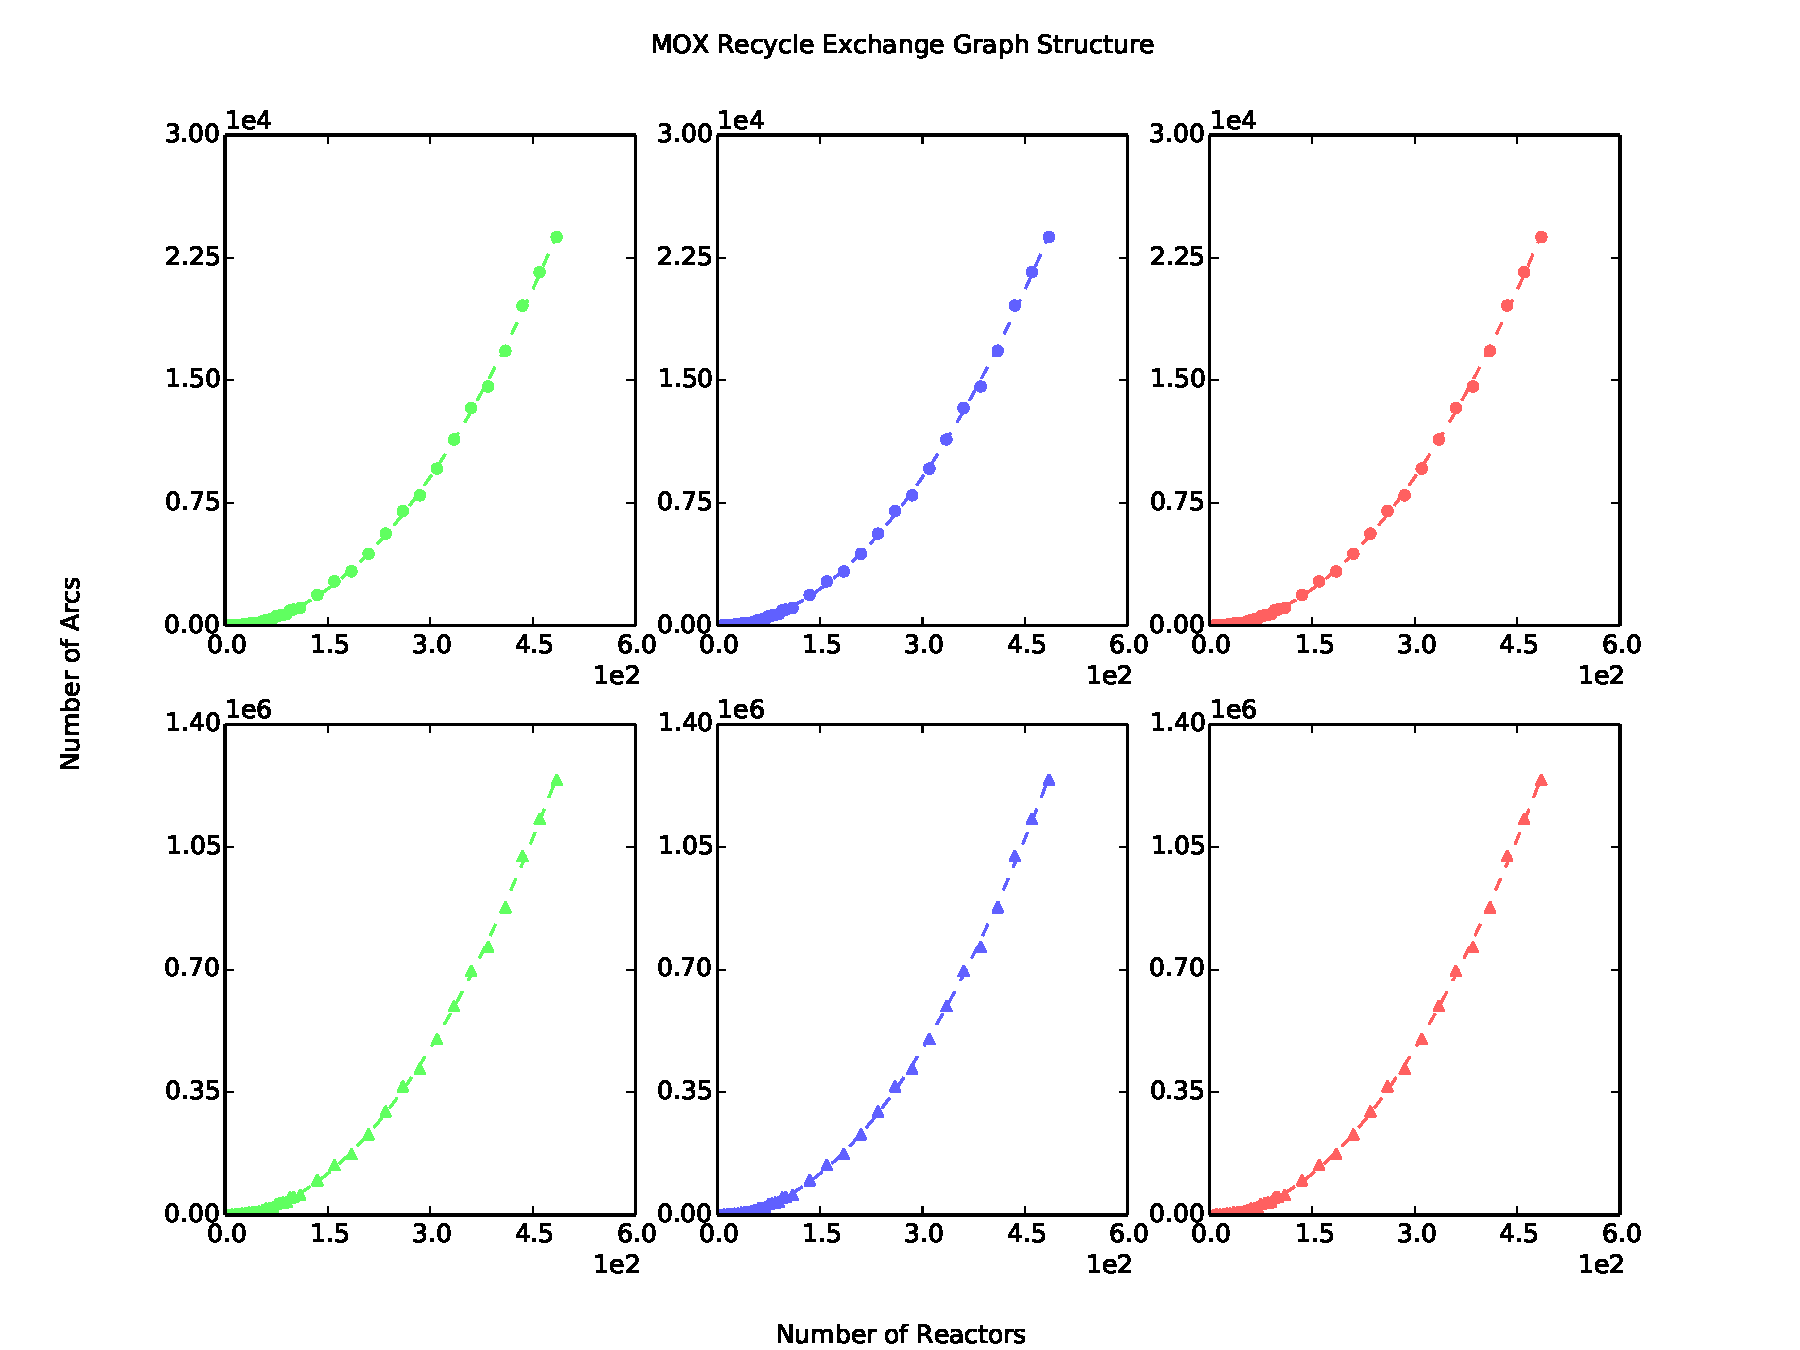
\includegraphics[width=.7\textwidth]{base_back_n_rxtr_n_arcs_fc1_greedy.pdf}
    \caption{
      \label{fig:base_back_n_rxtr_n_arcs_fc1_greedy}
      Arc population scaling with the number of reactors with corresponding linear fits.}
  \end{center}
\end{figure}

\subsubsection{Reference Case}

\paragraph{Greedy Solver}

The Greedy solver performs quite similarly to the front-end case. Its
performance is again linear-like in the number of arcs. An example of the MOX
fuel cycle is shown in Figure \ref{fig:base_back_n_arcs_time_fc1_greedy}. As can
be seen, the linear coefficient in back-end cases is approximately twice the
coefficient of front-end cases. This observation holds irrespective of fuel
cycle.

\begin{figure}[h!]
  \begin{center}
    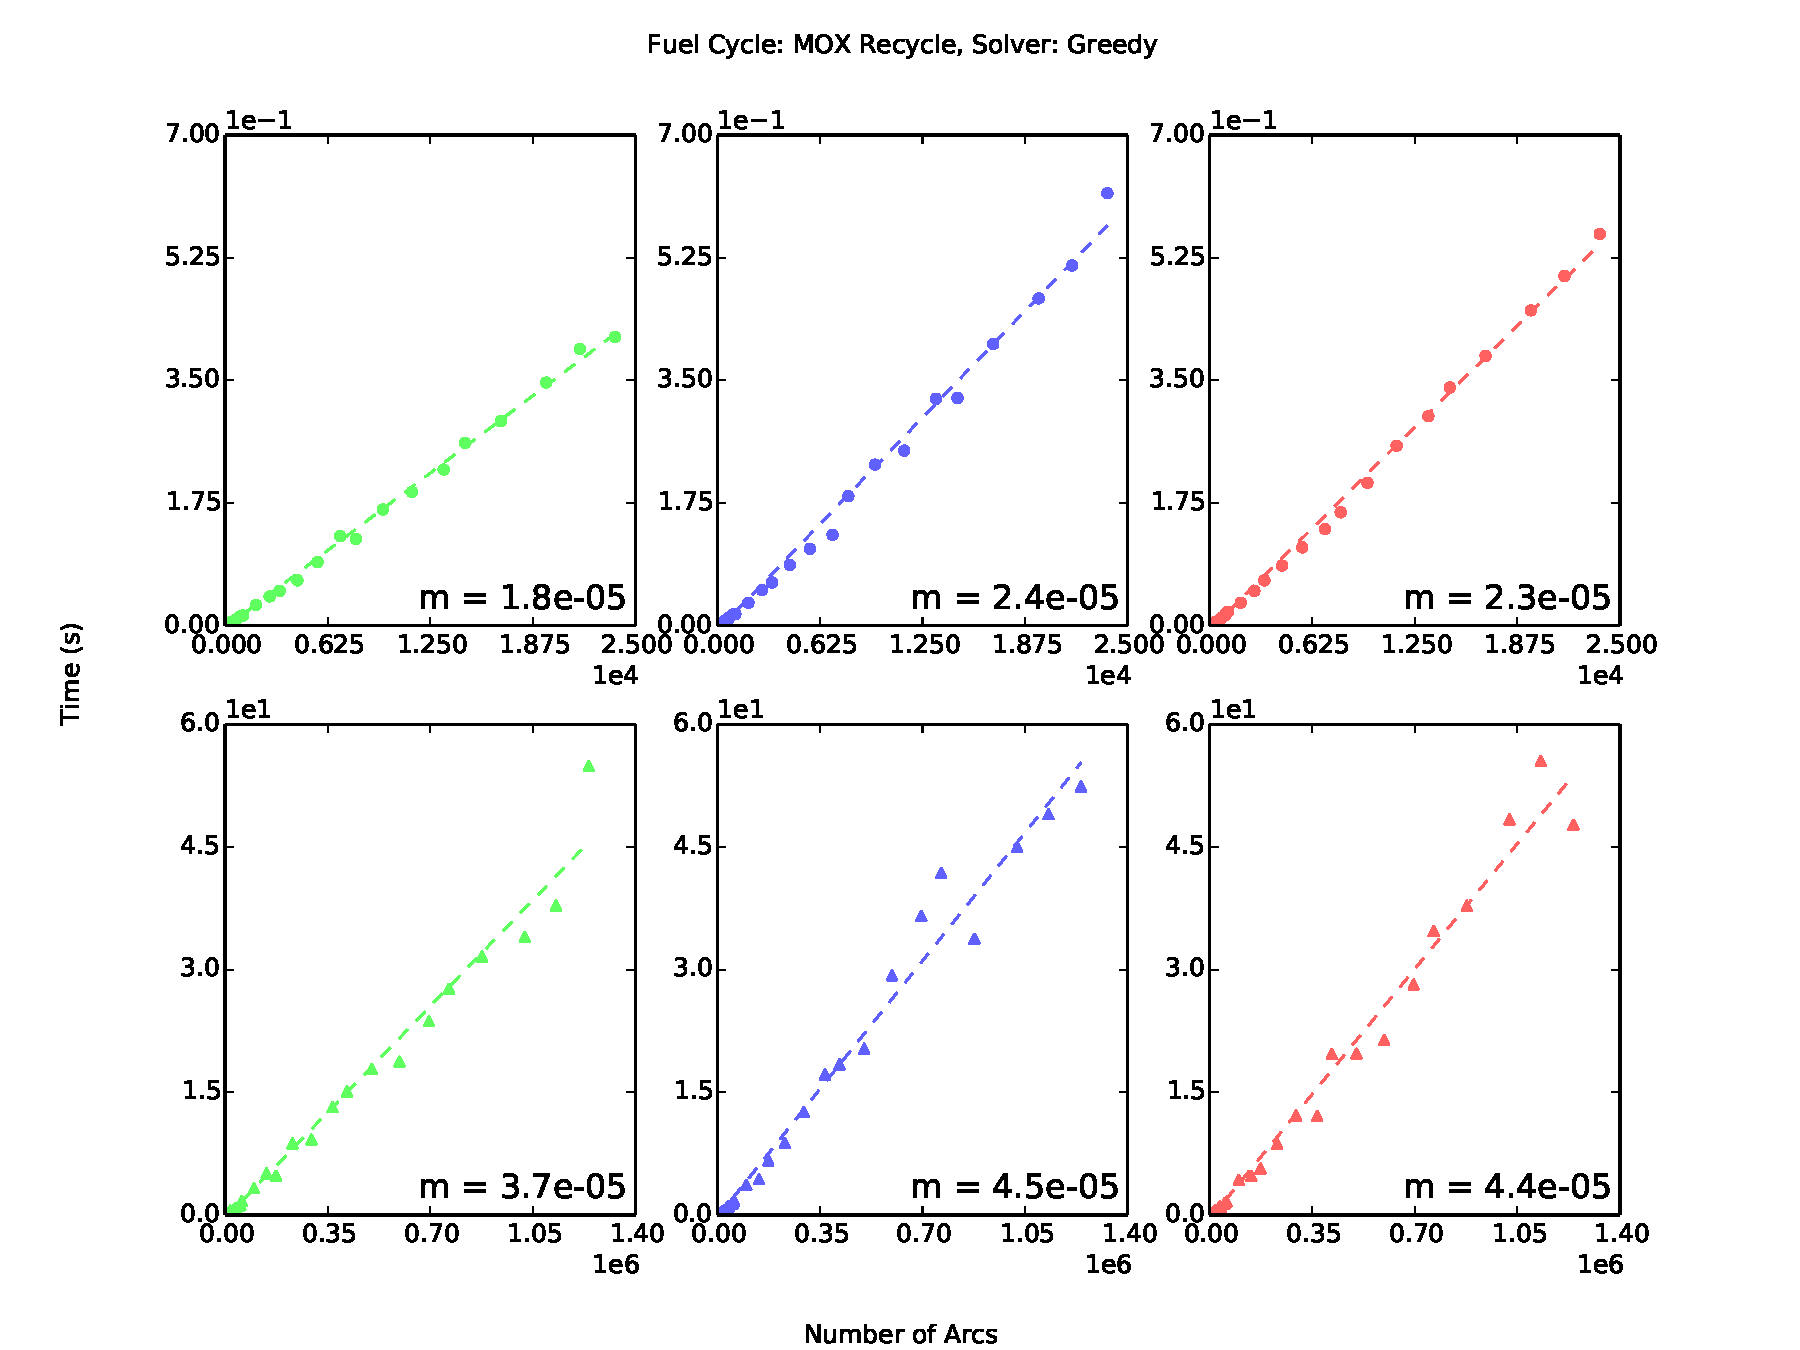
\includegraphics[width=.7\textwidth]{base_back_n_arcs_time_fc1_greedy.pdf}
    \caption{
      \label{fig:base_back_n_arcs_time_fc1_greedy}
      Greedy Solver results for the MOX fuel cycle as the number of arcs
      increases.      
    }
  \end{center}
\end{figure}

\paragraph{CLP Solver}

Back-end exchanges solved with \clp were found to behave similarly for each fuel
cycle modeled. The results for MOX-based exchanges is shown in
\ref{fig:base_back_n_constrs_time_fc1_clp} with quadratic fits. A key distinction
is observed between back-end and front-end exchanges: while front-end exchanges
follow tight $\mathcal{O}(n^2)$ scaling in all cases, back-end exchanges with
higher-reactor fidelity clearly have a larger spread in this trend. Furthermore,
significantly higher run times are observed for back-end exchanges, with a
maximum run time of $\sim$40 seconds for front-end exchanges and $\sim$150-300
seconds for back-end exchanges.

\begin{figure}[h!]
  \begin{center}
    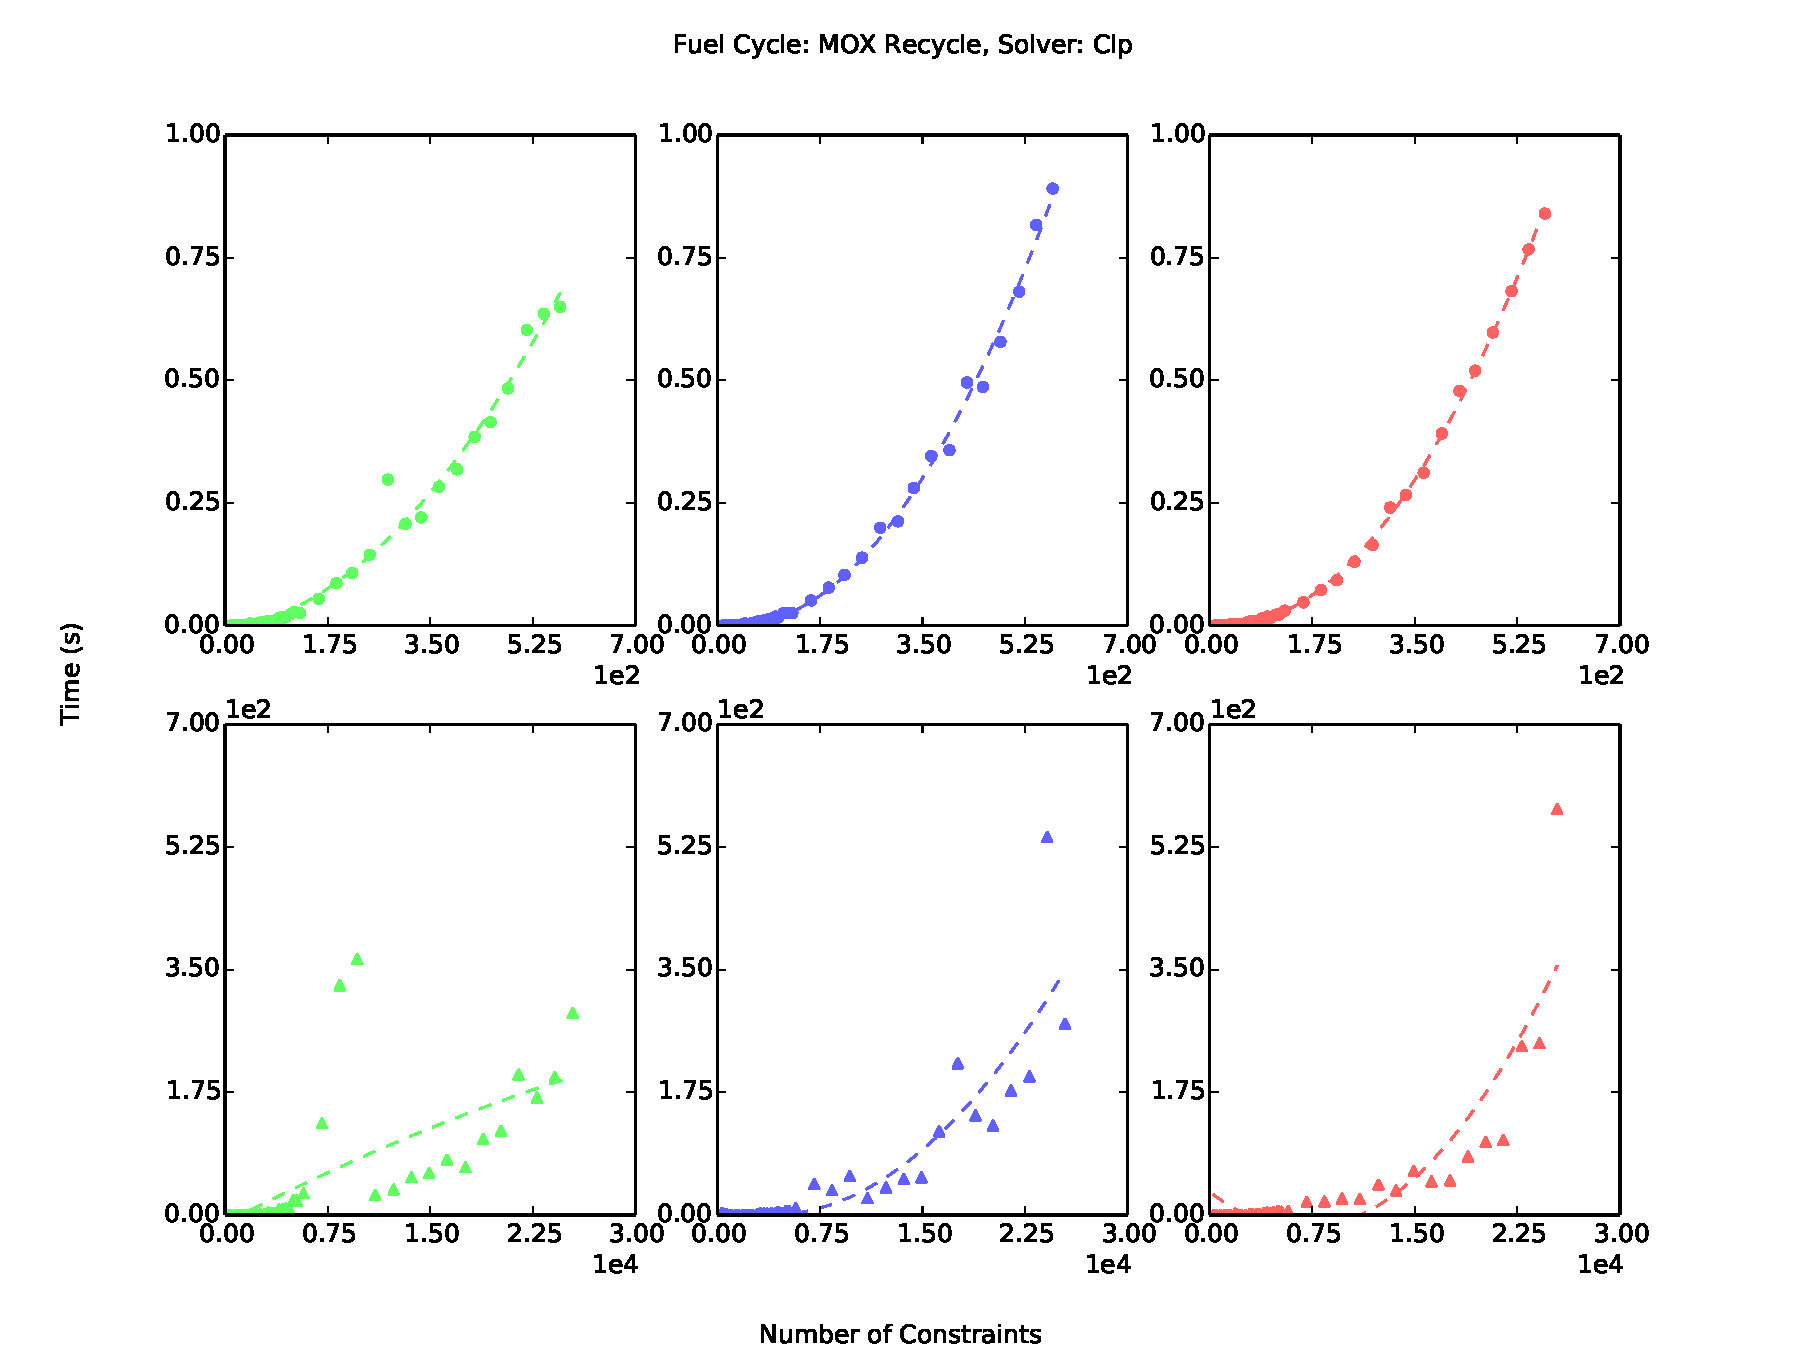
\includegraphics[width=.7\textwidth]{base_back_n_constrs_time_fc1_clp.pdf}
    \caption{
      \label{fig:base_back_n_constrs_time_fc1_clp}
      \clp Solver results for the MOX fuel cycle as the number of constraints
      increases.      
    }
  \end{center}
\end{figure}

\paragraph{\cbc Solver}

\cbc behavior is also similar to the front-end case. Importantly, exponential
scaling with problem size is again apparent, as can be seen in Figure
\ref{fig:base_back_n_arcs_time_fc1_cbc}. The primary difference between the two
exchange types is the increased population of converged solutions for
high-fidelity reactor instances. Whereas reactor fidelity was not a large factor
with respect to convergence probability in front-end exchanges, it appears to be
a large factor for back-end exchanges.
 
\begin{figure}[h!]
  \begin{center}
    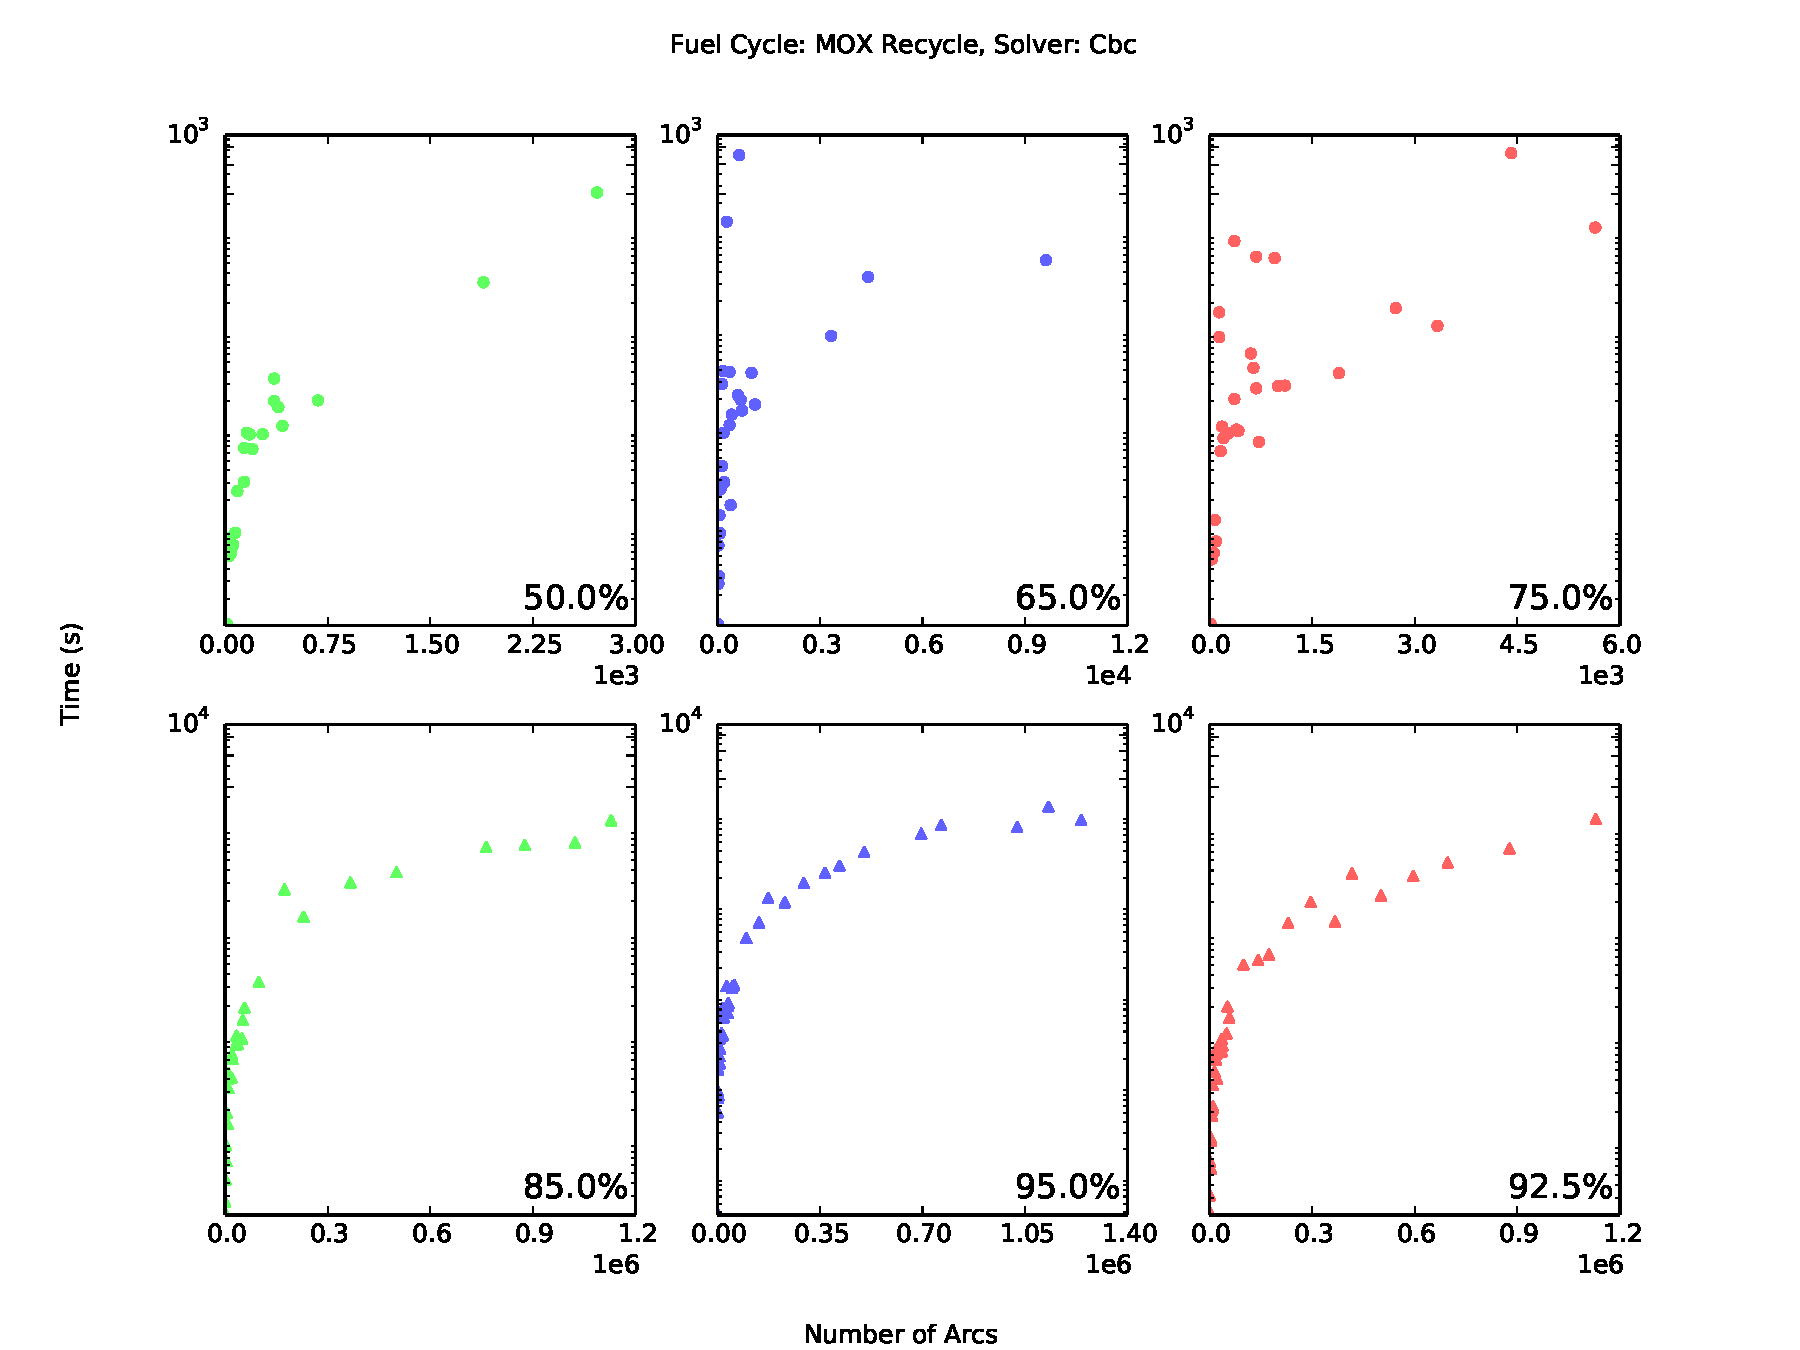
\includegraphics[width=.7\textwidth]{base_back_n_arcs_time_fc1_cbc.pdf}
    \caption{
      \label{fig:base_back_n_arcs_time_fc1_cbc}
      \cbc Solver results for the MOX fuel cycle as the number of arcs
      increases.      
    }
  \end{center}
\end{figure}

\subsubsection{Solution Comparison}\label{sec:res:scale:front:soln}

Two notable features can be seen when comparing Greedy and \cbc solutions in
Figure \ref{fig:compare_cbc_greedy_pref_flow_back_n_rxtr__fc1_}. The first is
that \cbc almost always performs better than Greedy in preference space. Further,
$z^*_{\text{sim}} \leq z_{\text{sim}, \text{Greedy}}$ is true only for very
small exchanges. Additionally, \cbc preference space results relative to the
Greedy solver are, in general, better for low-fidelity reactor exchanges than
high-fidelity exchanges.

Secondly, the simulation-objective gain from using \cbc appears to be
problem-size independent when there are a large number of variables in back-end
exchanges. As can be seen high-fidelity reactor results in Figure
\ref{fig:compare_cbc_greedy_pref_flow_back_n_rxtr__fc1_}, when the number of
reactors is large, a relative gain in simulation objective of 30\%-40\% is
realized by using \cbc. The final value is a function of the degree to which
location-based preferences are used.

\begin{figure}[h!]
  \begin{center}
    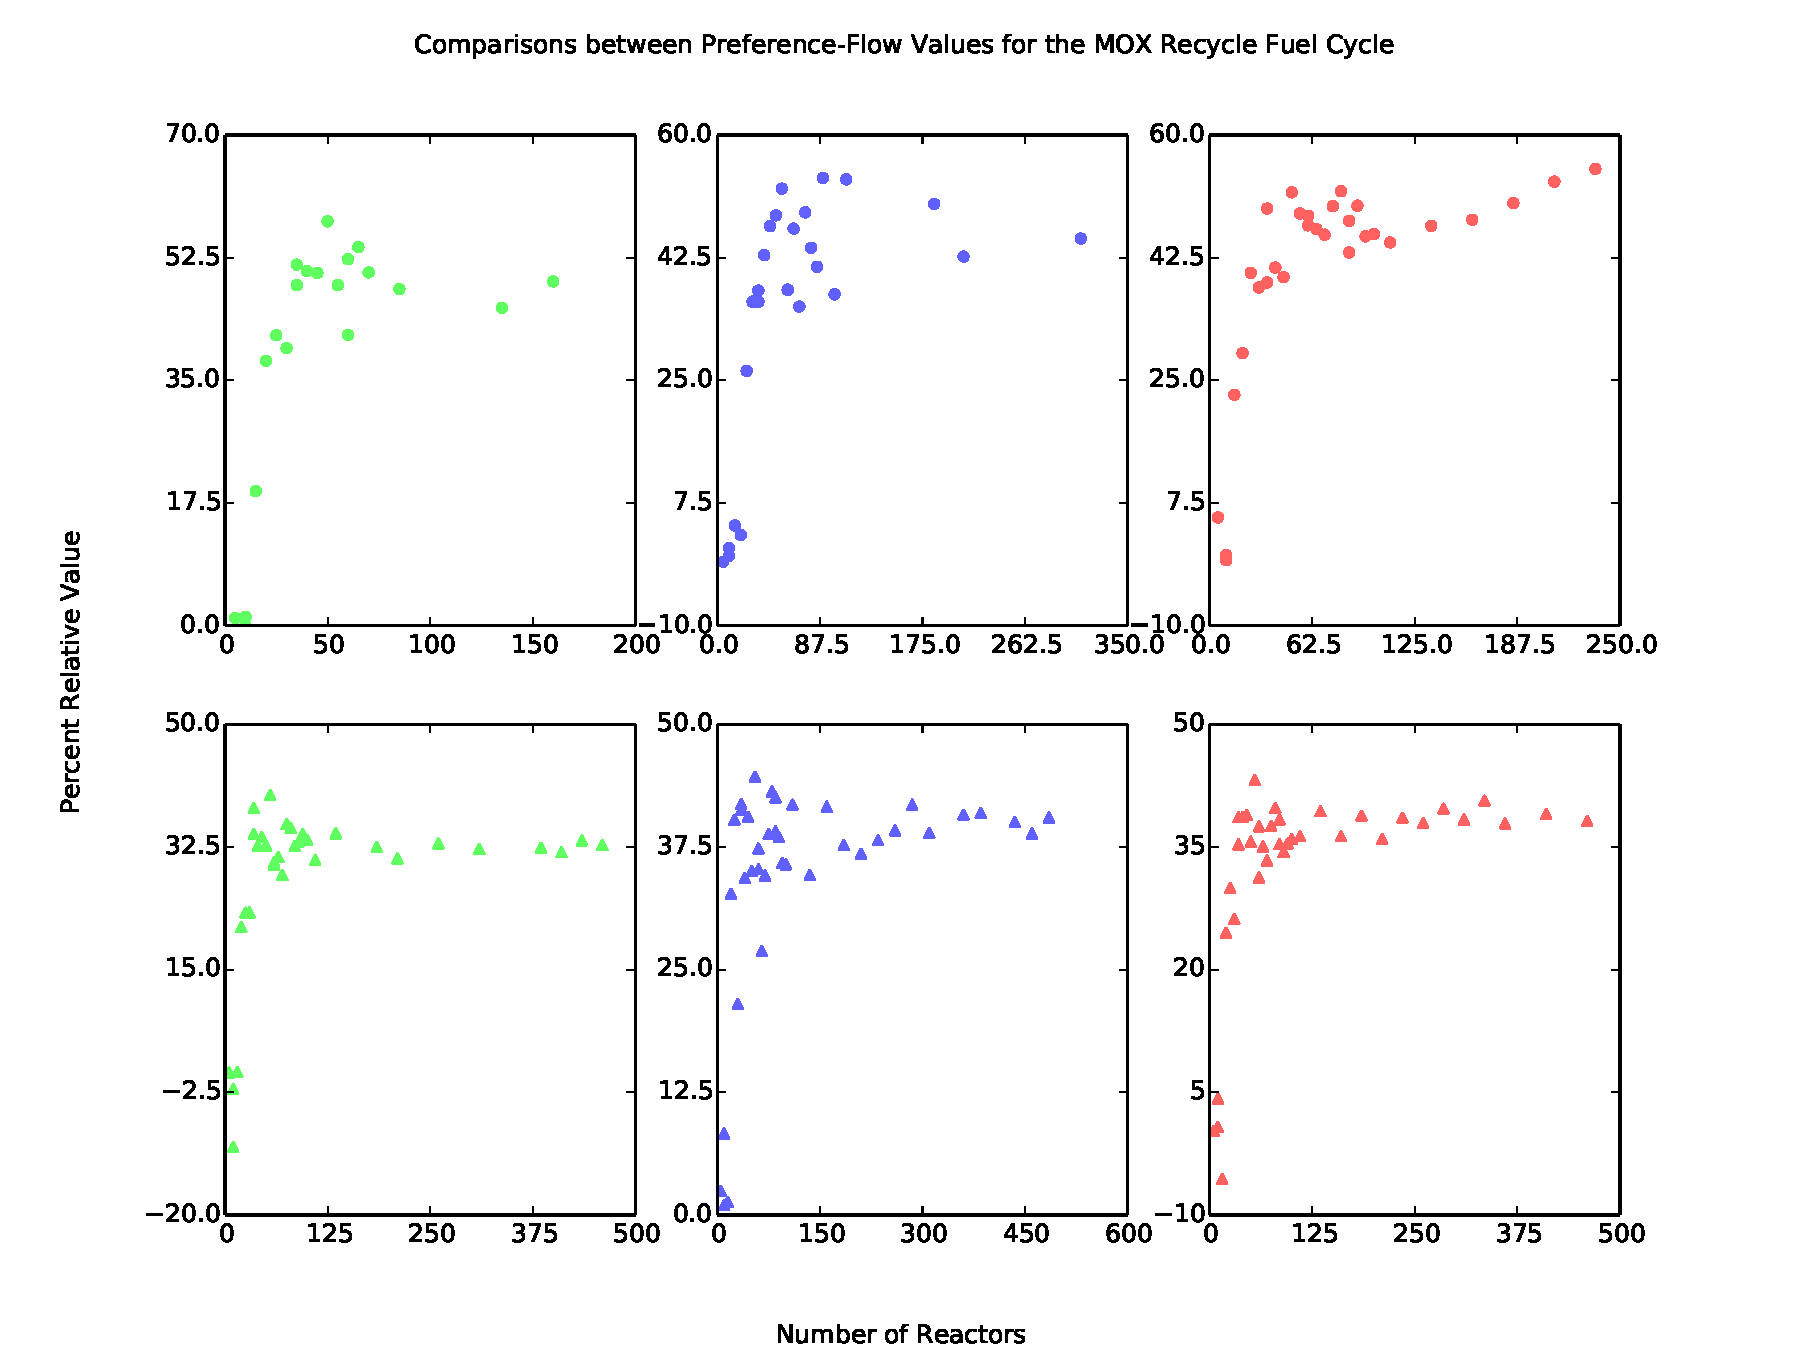
\includegraphics[width=.7\textwidth]{compare_cbc_greedy_pref_flow_back_n_rxtr__fc1_.pdf}
    \caption{
      \label{fig:compare_cbc_greedy_pref_flow_back_n_rxtr__fc1_}
      Comparisons between relative simulation metrics between the \cbc solver and
      the Greedy solver for MOX fuel cycles. Only converged \cbc
      solutions are compared.  }
  \end{center}
\end{figure}
